\documentclass{article}
\usepackage{amssymb,lineno}
\modulolinenumbers[5]
\usepackage{color}
\usepackage[colorlinks,linkcolor=black,hyperindex,CJKbookmarks,dvipdfm]{hyperref}
\usepackage{tikz}
\usetikzlibrary{arrows,shapes,chainsexit}
\usetikzlibrary{shapes.geometric}
\usetikzlibrary{arrows.meta}
\usepackage{authblk}
\usepackage{graphics,graphicx}
\usepackage{mathrsfs}
\usepackage{amsmath,bm}
\usepackage{subfigure}
\usepackage{booktabs}
\usepackage{amsthm}
\usepackage{subfigure}
\usepackage{listings}
\usepackage{setspace}
\usepackage[margin=2.5cm]{geometry}
\usetikzlibrary{shapes.geometric, arrows.meta,matrix,positioning,calc}
\intextsep=8pt plus 3pt minus 1pt
\definecolor{ColorMark}{rgb}{1,1,1}
\numberwithin{equation}{section}
\numberwithin{table}{section}
\graphicspath{{picture/}}
\bibliographystyle{elsarticle-num}

\begin{document}

\title{A multi-material HLLC Riemann solver with both elastic and plastic waves for 1D  elastic-plastic flows}
\author{Li Liu$^1$,Junbo Cheng $^{1,*}$, Jiequan Li}
%\cortext[mycorrespondingauthor]{
%Correspondence to: Junbo Cheng, Institute of Applied Physics and Computational Mathematics, Beijing 100094, China. E-mail: Cheng\_junbo@iapcm.ac.cn}

\maketitle

%\address{$^1$  Institute of Applied Physics and Computational Mathematics, Beijing 100094, China }

\begin{abstract}
  A multi-material HLLC-type  approximate Riemann solver with both the elastic and plastic waves (MHLLCEP) is constructed for 1D elastic-plastic flows with a hypo-elastic constitutive model and the von Mises yielding condition. Comparing with the HLLCE Riemann solver introduced in Cheng, during constructing MHLLCEP, we do not use any assumption and so describe and evaluate the plastic waves more accurate than do in HLLCE. Moreover, if the non-linear waves in the Riemann problem are only shock waves, even with the plastic waves, MHLLCEP is accurate. Based on MHLLCEP, combining with the third-order WENO reconstruction method and the third-order Runge-Kutta method in time, a high-order cell-centered Lagrangian scheme for 1D elastic-plastic flows is built in this paper. A number of numerical experiments are carried out and numerical results showed the presented third-order scheme is convergent, stable, and essentially non-oscillatory. Moreover, for multi-material elastic-plastic flows, the scheme with MHLLCEP is more accurate and more reasonable in resolving the multi-material interface than the scheme with HLLCE.
\end{abstract}

%\begin{keyword}
%  HLLC Riemann solver with elastic and plastic waves, high-order cell-centered Lagrangian scheme,  WENO scheme,  hypo-elastic constitutive model, elastic-plastic flows
%\end{keyword}

\section{Introduction}

In this paper, a multi-material elastic-plastic HLLC-type approximate Riemann solver(MHLLCEP) is developed, with the capability of resolving both elastic and plastic waves, to simulate one-dimensional  multi-material elastic-plastic solid problems with the isotropic elastic-plastic model \cite{wilkins1963calculation} and von Mises' yielding condition in the framework of high-order cell-centered Lagrangian scheme.

Generally, elastic-plastic flows can be mainly simulated in three ways, Eulerian method \cite{trangenstein1991higher,miller2001high,barton2009exact}, staggered Lagrangian schemes \cite{wilkins1963calculation} and cell-centered Lagrangian schemes \cite{burton2013cell,kluth2010discretization,maire2013nominally,cheng2017third} which is considered in this paper.
Cell-centered Lagrangian  scheme  is derived  based on the Godunov methods and has combined many advantages from both staggered Lagrangian schemes and Eulerian methods. Firstly, it's no necessary to use artificial viscosity  which always is used in the staggered Lagrangian schemes; Secondly, it is easy to guarantee the total energy conservation; Besides, it can also be used to simulate the problems with both  hyper-elastic and hypo-elastic models  \cite{burton2013cell,kluth2010discretization,maire2013nominally,cheng2017third}  as a Lagrangian scheme.

In the  Godunov-type method,  a core process is to construct the conservative flux by solving a Riemann problem  at each cell face. As the Riemann problem contains many physical structures, especially in elastic-plastic flows, such as elastic waves, plastic waves and contact waves or interfaces between different materials, the property of the approximate Riemann solver may do a magnitude influence in the simulation. Recently, there is a lot of works have been done in this area. For example, Gavrilyuk et al. \cite{gavrilyuk2008modelling} analyzed the structure of Riemann solution to construct a Riemann solver for the linear elastic system  of hyperbolic non-conservative models for transverse waves, wherein an extra evolution equation was added in order to make the elastic transformations reversible in the absence of shock waves. Despres \cite{despres2007geometrical} built a shock solution to a non-conservations reversible system of hypo-elasticity models and found that a sonic point is necessary to construct compression solution that begins at a constrained compressed state.  Cheng eta al.  \cite{cheng2015high} analyzed the wave structures of one-dimensional elastic-plastic flows and developed an effective two-rarefaction approximate Riemann solver with elastic waves (TRRSE) and build the second-order and third-order cell-centered Lagrangian schemes based on the TRRSE, but the TRRSE is a little  expensive as iteration method is used in it.
In \cite{cheng2016harten}, for one-dimensional elastic-plastic flows, Cheng introduced a HLLCE Riemann solver, which is fast and efficient in resolving elastic waves and plastic waves for numerical examples in \cite{cheng2016harten}, but Cheng evaluated the deviatoric stresses from the following \emph{assumption: a pressure is continuous across the contact wave} in the Riemann solver. This assumption is valid for pure fluids, but for elastic-plastic flows, this assumption maybe lead to some errors. There are three cases we need  to consider.
\begin{enumerate}
  \item If both states in the star regions between the contact wave are elastic, this assumption does not results in errors;
  \item If the both states reach the elastic limit, there are two cases we need take into account:
  \begin{enumerate}
    \item if the both materials across the interface are same, this assumption does not results in errors, too;
    \item if the both materials are different, this assumption will result in big errors because the yielding strengths of different materials are always different;
  \end{enumerate}
  \item If one state in one side of the interface are yielded, but another does not,  this assumption also results in big errors.
\end{enumerate}

For the above consideration, in this paper, we aim to construct a new HLLC-type Riemann solver which is suitable for 1D multi-material elastic-plastic flows. In the new solver, both the elastic waves and plastic waves are resolved and the assumption in \cite{cheng2016harten} that the pressure is continuous across the interface is deleted; Correspondingly, the errors introduced by the assumption will also be eliminated.

Combined with an improved third-order WENO scheme\cite{liu2018novel} and Runge-Kutta scheme, a high-order cell-centered Lagrangian scheme is given in this paper for one-dimensional multi-material elastic-plastic flows.

This paper is organized as follows. In section 2, we briefly introduce the governing equations to be studied. In section 3, the MHLLEP method is constructed.  Then, high-order elastic-plastic cell-centered Lagrangian schemes is given in section 4. Some numerical examples are presented to validate the method.  Conclusions are shown in section 5.
\section{Governing equations}

The equations for a continuous one-dimensional solid in differential form are given as

\begin{equation*}
\partial_t \mathbf{{U}} + \partial _x \bm{F}(\mathbf{{U}}) = 0, \   x \in \   \Omega \subset \mathbf{R}, \  t>0,
\end{equation*}
where
\begin{equation}
  \mathbf{U} = \left[ \begin{array}{l}
	  \rho \\
	  \rho u \\
	  \rho  E \\
	\end{array}
  \right],
  \hspace{0.3cm}
  \mathbf{F} = \left[ \begin{array}{l}
	  \rho u \\
	  \rho u^2 -\sigma_x\\
	  (\rho E -\sigma_x)u\\
  \end{array} \right],
\end{equation}
$\rho$, $u$, $\sigma_x$ and $E$ are  the density, velocity in $x-$direction, Cauchy stress and total energy per unit volume, respectively, $E$ has the relation with specific internal energy $e$ as
\begin{equation}
  E = e+\frac{1}{2}u^2,
\end{equation}
\begin{equation}
  \sigma_x = -p +s_{xx},
\end{equation}
where $p$ and $s_{xx}$ denote hydrostatic pressure and deviatoric stress in the $x-$ direction, respectively.

In this paper, the elastic energy is not included in the total energy. The exclution of the elastic energy is usual for practical engineering problems \cite{maire2013nominally} and is different from that in Ref.\cite{gavrilyuk2008modelling}.

The relation of the pressure with  the density and the specific internal energy is gotten from the equation of state (EOS). In this paper, we consider the Mie-Gr\"uneisen EOS,
\begin{equation}\label{eq:mie}
  p(\rho,e) = \rho_0 a_0^2f(\eta)+ \rho_0 \Gamma_0 e,
\end{equation}
where $f(\eta) = \frac{(\eta-1)(\eta-\Gamma_0(\eta-1)/2)}{(\eta-s(\eta-1))^2}$, $\eta = \frac{\rho}{\rho_0}$, $\rho_0$, $a_0$, $s$, and $\Gamma_0$ are constant parameters of the Mie-Gr\"uneisen EOS.

Hooke's law is used here to describe the relationship between the deviatoric stress and the strain,
\begin{equation}\label{eq:sxx1}
\dot{s}_{xx} = 2\mu \left(\dot{\varepsilon}_x-\frac{1}{3}\frac{\dot{V}}{V}\right),
\end{equation}
where $\mu$ is the shear modulus, $V$ is the volume, and the dot means the material time derivative,
\begin{equation}\label{eq:mt}
  \dot{()} = \frac{\partial ()}{\partial t} + u \frac{\partial ()}{\partial t},
\end{equation}
and
\begin{equation}\label{eq:vare}
  \dot{\varepsilon}_x = \frac{\partial u}{\partial x}, \hspace{0.3cm} \frac{\dot{V}}{V} = \frac{\partial u}{\partial x}.
\end{equation}

By using Eq.(\ref{eq:vare}), Eq.(\ref{eq:sxx1}) can be rewritten as
\begin{equation}\label{eq:sxx}
  \frac{\partial s_{xx}}{\partial t} + u \frac{\partial s_{xx}}{\partial t} =\frac{4}{3}\mu \frac{\partial u}{\partial x}.
\end{equation}

The Von Mises' yielding condition is used here to describe the elastic limit. In one spatial dimension, the von Mises' yielding criterion is given by
\begin{equation}
  |s_{xx}| \le \frac{2}{3}Y_0,
\end{equation}
where $Y_0$ is the yield strength of the material in simple tension.

\section{MHLLCEP}\label{sec:HLLCEP}
\subsection{The Riemann problem}

The Riemann problem for the 1D time dependent elastic-plastic equations is given as follows:
 \begin{equation}\label{eq:1d}
   \left\{ \begin{aligned}
	   & \partial _t \rho +\partial_x(\rho u)=0,\\
	   & \partial _t (\rho u)+\partial_x(\rho u^2 + p -s_{xx})=0,\\
	   &\partial _t (\rho E)+\partial_x\left[(\rho E + p -s_{xx})u\right]=0,\\
	   &\partial _t s_{xx}+u\partial_xs_{xx}-\frac{4}{3}\partial_x u=0,\\
& |s_{xx}|\leq \frac{2}{3}Y_{0}, \\
	   &Q(x,t = 0) = \left\{\begin{aligned}
		   Q_L, \hspace{0.1cm} \text{if} \hspace{0.1cm} x<0, \\
		   Q_R, \hspace{0.1cm} \text{if} \hspace{0.1cm} x\ge 0, \\
	   \end{aligned}\right.
	 \end{aligned}
  \right.
\end{equation}
where $Q = (\rho, \rho u, \rho E, s_{xx})^T$.

\subsection{Jacobian matrix} %and the eigenvalues and eigenvectors}
For the Mie-Gr\"uneisen EOS, the system (\ref{eq:1d}) can be written as
\begin{equation}
  \partial _t \bm{Q} +\bm{J}(\bm{Q})\partial_x\bm{Q} = 0,
\end{equation}
where
\begin{equation}\label{eq:Jcb}
  J = \left[\begin{array}{llll}
	  0 & 1 & 0 & 0 \\
	  -u^2 + \frac{\partial p}{\partial \rho} +\Gamma(\frac{u^2}{2}-e)& u(2-\Gamma)& \Gamma & -1 \\
	  (\Gamma(\frac{u^2}{2}-e)-e+\frac{\sigma_x}{\rho}+\frac{\partial p}{\partial \rho})u & -\Gamma u^2 -\frac{\sigma_x}{\rho} +e & (1+\Gamma)u& -u\\
	\frac{4}{3}\mu\frac{u}{\rho} & -\frac{4}{3}\mu\frac{1}{\rho}& 0 & u \\
\end{array}
\right],
\end{equation}
where $\Gamma = \frac{\Gamma_0\rho_0}{\rho} $.

The eigenvalues of the coefficient matrix $\bm{J}(\bm{Q})$ are given as
\begin{equation}
  \lambda_1 =\lambda_2 = u, \hspace{0.3cm} \lambda_3 = u-c, \hspace{0.3cm} \lambda_4 = u+c,
\end{equation}
where
\begin{equation}
  \left\{ \begin{aligned}
	  & c = \sqrt{a^2-\frac{\rho_0}{\rho^2}\Gamma_0 s_{xx} +\frac{4}{3}\frac{\mu}{\rho}},\\
	&	a^2 = \frac{\partial p}{\partial \rho} + \frac{p}{\rho^2}\frac{\partial p}{\partial e} = a^2_0 \frac{\partial f}{\partial \eta} + \frac{p}{\rho^2}\rho_0 \Gamma_0.
	  \end{aligned} \right.
	\end{equation}
The corresponding right eigenvectors are
\begin{equation}\label{eq:eiv}
  r_1 = \left[ \begin{array}{l}
	  \frac{1}{b_1} \\
	  \frac{u}{b_1} \\
	  0 \\
	  1 \\
	\end{array}
	\right], \hspace{0.2cm}
	r_2= \left[ \begin{array}{l}
		-\frac{\Gamma}{b_1} \\
		-\frac{\Gamma u}{b_1} \\
		1 \\
		0\\
	  \end{array}
	\right], \hspace{0.2cm}
r_3 =	\frac{1}{\phi^2}\left[\begin{array}{l}
		1 \\
		u-c \\
		h -uc \\
		\phi^2
	  \end{array}
	\right], \hspace{0.2cm}
r_4 = \frac{1}{\phi^2}\left[\begin{array}{l}
		1 \\
		u+c \\
		h +uc \\
		\phi^2
	  \end{array}
	\right],
  \end{equation}
  where
  \begin{equation}
	b_1 = \frac{\partial p}{\partial \rho} - \Gamma E,  \quad h = E +\frac{p-s_{xx}}{\rho},
  \end{equation}
  and
  \begin{equation}
	\phi^2 = a^2 -\frac{\rho_0}{\rho^2} \Gamma_0 s_{xx}-c^2 = -\frac{4\mu}{3}\frac{1}{\rho}.
  \end{equation}


\subsection{Formulations between the  contact wave or the interface}
  For  a  system without molercular diffusion, there is no materials convecting  cross the contact wave or interface, so the velocities between the discontinuity are always equal, $u_L^* = u_R^*$. This can also be verified by the eigenvectors  in Eq.(\ref{eq:eiv}).

  Using the eigenvectors in  Eq.(\ref{eq:eiv}), for the $\lambda_{1}$-wave we
have
\begin{equation}   \label{e23a}
\frac{d \rho}{\frac{1}{b_{1}}} = \frac{d \rho u}{\frac{u
}{b_{1}}}=\frac{d \rho E}{0} = \frac{d s_{xx}}{1}.
\end{equation}
From the above equations, we can easily deduce that
\begin{equation}   \label{e23b}
du = 0, \quad d(s_{xx}-p)=0,
\end{equation}
 which means
\begin{equation}   \label{e23c}
  u_{L}^{\ast}=u_{R}^{\ast},
\end{equation}
and
\begin{equation}   \label{e23d}
\sigma_{x,L}^{\ast}=\sigma_{x,R}^{\ast},
\end{equation}
where $()_{L}^{\ast}$ and $()_{R}^{\ast}$ denote $()$ in the region
of $\mathbf{W}_{L}^{\ast}$ and $\mathbf{W}_{R}^{\ast}$,
respectively. Here we do not show the details of the derivation for
simplicity of presentation.


Using the eigenvectors (\ref{eq:eiv}), for the $\lambda_{2}$-wave we
have
\begin{equation}   \label{e24a}
\frac{d \rho}{\frac{-\Gamma}{b_{1}}} = \frac{d \rho u}{\frac{-u
\Gamma}{b_{1}}}=\frac{d \rho E}{1} = \frac{d s_{xx}}{0}.
\end{equation}
From the above equations, we can easily deduce  that
\begin{equation}   \label{e24b}
du = 0, \quad dp=0, \quad ds_{xx}=0,
\end{equation}
 which means
\begin{equation}   \label{e24c}
  u_{L}^{\ast}=u_{R}^{\ast},
\end{equation}
\begin{equation}   \label{e24d}
p_{L}^{\ast}=p_{R}^{\ast}, \quad
  s_{xx,L}^{\ast}=s_{xx,R}^{\ast},
\end{equation}
where $()_{L}^{\ast}$ and $()_{R}^{\ast}$ denote $()$ in the region
of $\mathbf{W}_{L}^{\ast}$ and $\mathbf{W}_{R}^{\ast}$,
respectively.

From  Eq.(\ref{e24d}), we  get that
\begin{equation}   \label{e27a}
\sigma_{x,L} ^{\ast}=  \sigma_{x,R} ^{\ast}.
\end{equation}


At last, for the $\lambda_{1}$ and $\lambda_{2}$ waves, one can find
that the following two equations always hold:
\begin{equation}   \label{e28}
u_{L}^{\ast}=u_{R}^{\ast}, \quad
\sigma_{x,L}^{\ast}=\sigma_{x,R}^{\ast}.
\end{equation}

Using  the Rankine-Hugoniot relations between the contact wave  or  the interface
\begin{equation}
	\bm{F}_R^* = \bm{F}_L^*+s^*(\bm{U}_R^*-\bm{U}_L^*),
\end{equation}
where $s^*$ denotes the velocity of the contact wave.

From the first and second components of the above system, one can get
\begin{align}
  & \rho_R^* u_R^*=\rho_L^* u_L^*+s^*(\rho_R^*-\rho_L^*),\\
  & \rho_R^* u_R^{*2}-\sigma^*_R=\rho_L^* u_L^{*2}-\sigma_L^*+s^*(\rho_R^* u_R^*-\rho_L^* u_L^*).
\end{align}
%take $u_L^* = u_R^*$ in, we can get
Generally, for convenience, we define
\begin{equation}\label{eq:contact}
  s^* = u_L^* = u_R^*. % \hspace{0.3cm} \sigma_L^* = \sigma_R^*.
\end{equation}

\subsection{A relation between $\rho$ and $s_{xx}$ in 1D elastic-plastic  equation system}

Thanks to (\ref{eq:mt}), from the 1D elastic-plastic  equations in Eq.(\ref{eq:1d}), the equations of the density and the deviatoric stress can be written as
  \begin{equation}\label{eq:d1}
	\frac{\partial u}{\partial x} = -\frac{1}{\rho}\frac{d\rho}{dt},
  \end{equation}
  and
  \begin{equation}\label{eq:s1}
	\frac{ds_{xx}}{dt}=\frac{4}{3}\mu\frac{\partial u}{\partial x}.
  \end{equation}

  Substituting (\ref{eq:d1}) into (\ref{eq:s1}) yields
%  We can get a relation of density and deviatoric stress,
  \begin{equation}
	\frac{ds_{xx}}{dt}=-\frac{4}{3}\mu \frac{1}{\rho}\frac{d\rho}{dt}.
\end{equation}
Take an integration,
\begin{equation}\label{eq:rhosxx}
  s_{xx1}=-\frac{4}{3}\mu\text{ln}(\frac{\rho_{1}}{\rho_{0}})+s_{xx0}.
\end{equation}
The subscripts $1$ and $0$ mean the states in front of and behind a wave, respectively.
This relation always holds if there is no yielding in the integration path.

\subsection{Building MHLLCEP}
%Although HLLCE Riemann solver can simulate the elastic-plastic flow effectively and efficiently without iterations, but the plastic structure is not considered in and  there are some assumptions that are not so reasonable, especially in the interface between different materials. For example, the normal stresses $\sigma_x$ are  always equavalent across the interface, but the pressures are not always equal, and the consequent evaluation of $\widetilde{s}^*$ may   be of large error.

Now we considered the constructing details of MHLLCEP. As left-going or right-going  plastic waves exist possibly, there may be three to five waves in the Riemann structure, which depends on the yielding state  on the left side and right side of the interface.

\subsubsection{Pre-evaluating the states without considering of plastic waves}\label{sec:case1}
At first we do not know whether the states in the star region around the contact wave reach the elastic limit, so firstly \emph{assume that there is no plastic wave in and the material is totally yielding or totally not yielding} (\textbf{Assumption} 1). Based on \textbf{Assumption} 1, by using the HLLC method, we can get the states in the star region of the Riemann structure showed in  Fig.\ref{fig:case1}. If the obtained state contains yielding process, we will consider the cases showed in Fig.\ref{fig:case2}-\ref{fig:case4}.

The Riemann structure of MHLLCEP in Fig.\ref{fig:case1} is given as follows,
\begin{equation}\label{eq:HLLCEP}
  \bm{U}^{\text{MHLLCEP}}_{\text{Case1}}(x,t) = \left\{ \begin{aligned}
		& \bm{U}_L, \hspace{0.3cm} \text{if} \hspace{0.3cm} \frac{x}{t}\le s_L, \\
		& \bm{U}_L^*, \hspace{0.3cm} \text{if} \hspace{0.3cm} s_L\le \frac{x}{t} \le s^*, \\
		& \bm{U}_R^*, \hspace{0.3cm} \text{if} \hspace{0.3cm} s^*\le \frac{x}{t} \le s_R,\\
		& \bm{U}_R, \hspace{0.3cm} \text{if} \hspace{0.3cm} \frac{x}{t}\ge s_R, \\
	  \end{aligned}
	\right.
  \end{equation}
  and the corresponding Eulerian numerical flux and Lagrangian numerical flux are
 \begin{equation}
	\bm{F}^{\text{Euler}}_{\text{Case1}}(x,t) = \left\{ \begin{aligned}
		& \bm{F}_L, \hspace{0.3cm} \text{if} \hspace{0.3cm} \frac{x}{t}\le s_L, \\
		& \bm{F}_L^*, \hspace{0.3cm} \text{if} \hspace{0.3cm} s_L\le \frac{x}{t} \le s^*, \\
		& \bm{F}_R^*, \hspace{0.3cm} \text{if} \hspace{0.3cm} s^*\le \frac{x}{t} \le s_R,\\
		& \bm{F}_R, \hspace{0.3cm} \text{if} \hspace{0.3cm} \frac{x}{t}\ge s_R, \\
	  \end{aligned}
	\right.
  \end{equation}
\begin{equation}
	\bm{F}^{\text{Lag}}_{\text{Case1}}(x,t) = \left\{ \begin{aligned}
		& \bm{f}_L^*, \hspace{0.3cm} \text{if} \hspace{0.3cm} s_*\ge \frac{x}{t},\\
		& \bm{f}_R^*, \hspace{0.3cm} \text{if} \hspace{0.3cm} s^*\le \frac{x}{t},\\
	  \end{aligned}
	\right.
  \end{equation}
where $s^*$ denotes the speed of the contact wave, $f=(0,p-s_{xx},(p-s_{xx})u)^{T}$.

According to the Rankine-Hugoniot conditions between left elastic wave, one can get
\begin{equation} \label{eq:RH1}
	\bm{F}_L^* = \bm{F}_L+s_L (\bm{U}_L^*-\bm{U}_L).
\end{equation}
The first and second components of the above system can be written as
\begin{equation} \label{eq:rhoLstar}
  \rho_L^* u_L^*=\rho_L u_L+s_L(\rho_L^*-\rho_L),
\end{equation}
and
\begin{equation}\label{eq:sigma}
  \rho_L^* u_R^{*2}-\sigma^*_L=\rho_L u_L^2-\sigma_L+s_L(\rho_L^* u_L^*-\rho_L u_L).
\end{equation}
Using the relation of $u_L^* =u_R^* = s^*$ in Eq.(\ref{eq:contact}), the speed of contact wave can be evaluated as
\begin{equation}
 \hat{s}^* = \frac{\sigma_L-\sigma_R+\rho_L u_L(s_L-u_L)-\rho_R u_R(s_R-u_R)}{\rho_L(s_L-u_L)-\rho_R(s_R-u_R)},
\end{equation}
the density is solved as
\begin{equation}\label{eq:rhoLs}
  \hat{\rho}_L^* = \frac{\rho_L(u_L-s_L)}{\hat{s}^*-s_L}.
\end{equation}
Similarly, the density behind the right elastic wave is
\begin{equation}\label{eq:rhoLs}
  \hat{\rho}_R^* = \frac{\rho_R(u_R-s_R)}{\hat{s}^*-s_R}.
\end{equation}

Thanks to Eq.(\ref{eq:rhosxx}),  the deviatoric stress is evaluated as
\begin{equation}  \label{sxx1}
  \hat{s}_{xxL}^*=-\frac{4}{3}\mu\text{ln}(\frac{\hat{\rho}_L^*}{\rho_L})+s_{xxL}, \quad   \hat{s}_{xxR}^*=-\frac{4}{3}\mu\text{ln}(\frac{\hat{\rho}_R^*}{\rho_R})+s_{xxR}.
\end{equation}

If the speeds of left and right elastic waves are given, we can evaluate all states in the star region between the contact wave. Here we define the speeds of left and right elastic waves as
	\begin{equation}\label{eq:sLR}
	  s_L = \text{min} (u_L-c_L, u_R-c_R, 0),  \quad s_R = \text{max}(u_L+c_L, u_R+c_R, 0).
	\end{equation}
%Based on the assumption above, as there is no plastic wave in, we can take the relation of Eq.(\ref{eq:rhosxx}), and 

Using the pre-evaluated values of $\hat{s}_{xxL}^*$ and $\hat{s}_{xxR}^*$ in (\ref{sxx1}), we can classify the true condition into the following four cases.


\subsubsection{Case 1: No plastic wave}\label{sec:case1}
%
If $|s_{xxL}|<\frac{2}{3}Y_0$ and $|\hat{s}_{xxL}^*| < \frac{2}{3}Y_0$, all the states in the left are not yielding and there is no plastic wave; similarly, If $|s_{xxL}| \ge \frac{2}{3}Y_0$ and $|\hat{s}_{xxL}^*| \ge  \frac{2}{3}Y_0$, all the states in the left are yielding, there is also plastic wave. All the same things happen in the right.
%The \textbf{Assumption} 1  holds in the left.
%Meanwhile, if $|s_{xxR}|<\frac{2}{3}Y_0$ and $|\hat{s}_{xxR}^*| < \frac{2}{3}Y_0$, Or $|s_{xxR}| \ge \frac{2}{3}Y_0$ and $|\hat{s}_{xxR}^*| \ge  \frac{2}{3}Y_0$, the assumption holds in the right. 
In this case, the structures  of the Riemann solver are showed in Fig.\ref{fig:case1}.

Then
\begin{align}
&  s^* = \hat{s}^*,\hspace{0.3cm} \rho^*_L = \hat{\rho}_L^*, \hspace{0.3cm} \rho_R^* = \hat{\rho}_R^*,\\
&  s_{xxL}^*  = \Upsilon(\hat{s}_{xxL}^*),\hspace{0.3cm} s_{xxR}^*  = \Upsilon(\hat{s}_{xxR}^*)
\end{align}
where,
\begin{equation}\label{eq:upsilon}
  \Upsilon(\omega) = \left\{ \begin{aligned}
	  &\omega, \  \text{if} \  |\omega| \le \frac{2}{3}Y_0,\\
	  &\frac{2}{3}Y_0,  \ \text{if} \  \omega > \frac{2}{3}Y_0,\\
	 &-\frac{2}{3}Y_0,  \  \text{if} \ \omega < -\frac{2}{3}Y_0.\\
 \end{aligned}\right.
 \end{equation}

 The Cauchy stresses are solved  by Eq.(\ref{eq:sigma}),
\begin{equation*}
  \sigma_L^*=\sigma_R^*=\sigma_L -\rho_L (s_L-u_L)(s^*-u_L).
\end{equation*}
 Then we can get the pressure by $p =s_{xx}-\sigma$.
\begin{equation}
  p_L^* = s_{xxL}^* - \sigma_L^*,  \  p_R^* = s_{xxR}^* - \sigma_R^*.
\end{equation}

\begin{figure}
  \centering
  \begin{tikzpicture}
	\draw [line width =1pt,-{Stealth[length=2.5mm]}] (0,0) -- (4,0) node[below]{$x$};
	\draw [line width =1pt] (-4,0) -- (0,0);
	\draw [line width =1pt,-{Stealth[length=2.5mm]}] (0,0) -- (0,4) node[left]{$t$};
	\draw [double](0,0) -- ([turn]165:3.5)   node [above]{Contact};
	\draw  (0,0) -- ([turn]135:3.5) node [above]{Right elastic};
	\draw  (0,0) -- ([turn]-135:3.5) node [above]{Left elastic} ;
	\node at (-1.3,0.5) {$\bm{Q}_L$};
	\node at (-0.6,1.2) {$\bm{Q}_L^*$};
	\node at (0.7,1.2) {$\bm{Q}_R^*$};
	\node at (1.3,0.5) {$\bm{Q}_R$};
\end{tikzpicture}
\caption{The  structures of HLLCEP method, case 1: without plastic wave.}
\label{fig:case1}
\end{figure}

 \subsubsection{Case 2:  with only  the left plastic wave}\label{sec:case2}
 If in the left, $|s_{xxL}| \le \frac{2}{3}Y_0 \le  |\hat{s}_{xxL}^*|$; but in the right, ($|s_{xxR}|<\frac{2}{3}Y_0$ and $|\hat{s}_{xxR}^*| < \frac{2}{3}Y_0$) or ($|s_{xxR}|\geq \frac{2}{3}Y_0$ and $|\hat{s}_{xxR}^*| \geq \frac{2}{3}Y_0$), there will be only one plastic wave which is in the left. Correspondingly, the Riemann structure of this case is showed in Fig.\ref{fig:case2}. We need to solve the yielding state of $\widetilde{\bm{Q}}_L$. The MHLLCEP is given as follows in this case,
 \begin{equation}\label{eq:HLLCEP2}
   \bm{U}^{\text{MHLLCEP}}_{\text{Case2}}(x,t) = \left\{ \begin{aligned}
	   & \bm{U}_L, \hspace{0.3cm} \text{if} \hspace{0.3cm} \frac{x}{t}\le \widetilde{s}_L, \\
		&  \widetilde{\bm{U}}_L, \hspace{0.3cm} \text{if} \hspace{0.3cm} \widetilde{s}_L\le \frac{x}{t} \le  s_L, \\
		&\bm{U}_L^*, \hspace{0.3cm} \text{if} \hspace{0.3cm} s_L\le \frac{x}{t} \le s^*, \\
		& \bm{U}_R^*, \hspace{0.3cm} \text{if} \hspace{0.3cm} s^*\le \frac{x}{t} \le s_R,\\
		& \bm{U}_R, \hspace{0.3cm} \text{if} \hspace{0.3cm} \frac{x}{t}\ge s_R, \\
	  \end{aligned}
	\right.
  \end{equation}
  and the corresonding Eulerian and Lagrangian numerical fluxes are
 \begin{equation}\label{eq:HLLCEP}
   \bm{F}^{\text{Euler}}_{\text{Case2}}(x,t) = \left\{ \begin{aligned}
	   & \bm{F}_L, \hspace{0.3cm} \text{if} \hspace{0.3cm} \frac{x}{t}\le \widetilde{s}_L, \\
		&  \widetilde{\bm{F}}_L, \hspace{0.3cm} \text{if} \hspace{0.3cm} \widetilde{s}_L\le \frac{x}{t} \le   s_L , \\
		&\bm{F}_L^*, \hspace{0.3cm} \text{if} \hspace{0.3cm} s_L\le \frac{x}{t} \le s^*, \\
		& \bm{F}_R^*, \hspace{0.3cm} \text{if} \hspace{0.3cm} s^*\le \frac{x}{t} \le s_R,\\
		& \bm{F}_R, \hspace{0.3cm} \text{if} \hspace{0.3cm} \frac{x}{t}\ge s_R, \\
	  \end{aligned}
	\right.
  \end{equation}
\begin{equation}
	\bm{F}^{\text{Lag}}_{\text{Case2}}(x,t) = \left\{ \begin{aligned}
		& \bm{f}_L^*, \hspace{0.3cm} \text{if} \hspace{0.3cm} s_*\ge \frac{x}{t},\\
		& \bm{f}_R^*, \hspace{0.3cm} \text{if} \hspace{0.3cm} s^*\le \frac{x}{t}.\\
	  \end{aligned}
	\right.
  \end{equation}

 According to the Rankine-Hugoniot relation for the left  plastic wave, one get
  \begin{align}
	&\widetilde{\rho}_L(\widetilde{u}_L-\widetilde{s}_L) = \rho_L(u_L-\widetilde{s}_L), \label{eq:RHp1}\\
	&\widetilde{\rho}\widetilde{u}_L(\widetilde{u}_L-\widetilde{s}_L) = \rho_Lu_L(u_L-\widetilde{s}_L)+\widetilde{\sigma}_L-\sigma_L,  \label{eq:RHp2}\\
	&\widetilde{\rho}\widetilde{E}_L(\widetilde{u}_L-\widetilde{s}_L) = \rho_LE_L(u_L-\widetilde{s}_L)+\widetilde{\sigma}_L \widetilde{u}_L-\sigma_Lu_L, \label{eq:RHp3}
\end{align}
where $\widetilde{s}_L$ denotes the speed of left plastic wave.

Because the deviatoric stress behind the plastic wave reaches the elastic limit, the deviatoric stress and density are taken as
\begin{equation}
  \widetilde{s}_{xxL} =\left\{ \begin{aligned}
	  -\frac{2}{3}Y_0, \hspace{0.3cm} \text{if} \hspace{0.3cm} \rho_L^* > \rho_L,\\
	  \frac{2}{3}Y_0, \hspace{0.3cm} \text{if} \hspace{0.3cm} \rho_L^* < \rho_L,\\
	\end{aligned}\right.
  \end{equation}
  and
\begin{equation}   \widetilde{\rho}_{L} = \left\{ \begin{aligned}
	  & \rho_L \text{exp}\left(\frac{Y_0}{2\mu}+\frac{3 s_{xxL}}{4\mu}\right)  \hspace{0.5cm} \text{if} \hspace{0.3cm} \rho_L^* > \rho_L,\\
& \rho_L \text{exp}\left(-\frac{Y_0}{2\mu}+\frac{3 s_{xxL}}{4\mu}\right)
\hspace{0.3cm} \text{if} \hspace{0.3cm} \rho_L^* < \rho_L.\\
  \end{aligned}\right.
 \end{equation}

 The unknowns are the wave speed $\widetilde{s}_L$,  the velocity  $\widetilde{u}_L$, the pressure $\widetilde{p}_L$ and the specific internal energy $\widetilde{E}_L$. In the following, we will give the derivations of them.

 From Eq.(\ref{eq:RHp1}) we can get the wave speed as
  \begin{equation}
	\widetilde{s}_L = \frac{\widetilde{\rho}_L \widetilde{u}_L-\rho_Lu_L}{\widetilde{\rho}_L-\rho_L},
  \end{equation}
and  have the relation of
\begin{equation}\label{eq:u1_s}
  u_L-\widetilde{s}_L = \frac{(u_L-\widetilde{u}_L)\widetilde{\rho}_L}{\widetilde{\rho}_L-\rho_L}.
\end{equation}
Substituting Eq.(\ref{eq:RHp1}) into Eq.(\ref{eq:RHp2}), we have
\begin{equation}\label{eq:rho1}
  \rho_L(\widetilde{u}_L - u_L)(u_L-\widetilde{s}_L) = \widetilde{\sigma}_L -\sigma_L,
\end{equation}
then substituting Eq.(\ref{eq:u1_s}) into it, we can get the following relation
\begin{equation}\label{eq:tu_2}
  -t(\widetilde{u}_L-u_L)^2 = \widetilde{\sigma}_L-\sigma_L,
\end{equation}
where
\begin{equation}
t=\frac{\rho_L \widetilde{\rho}_L}{\widetilde{\rho}_L-\rho_L}.
\end{equation}
Similar to Eq.(\ref{eq:rho1}), Eq.(\ref{eq:RHp2}) can be changed into
\begin{equation}
  t(u_L-\widetilde{u}_L)(\widetilde{E}_L-E_L) =\widetilde{\sigma}_L\widetilde{u}_L-\sigma_Lu_L,
\end{equation}
and we also know that $E = e+\frac{1}{2}u^2$, then we have
\begin{equation}\label{eq:e21}
  \widetilde{e}_L-e_L= -\frac{\sigma_L+\widetilde{\sigma}_L}{2t}.
\end{equation}
The EOS (\ref{eq:mie}) can be written as
\begin{equation} \label{eq:eos1}
  e=c_0 p-c_1f(\rho/\rho_0),
\end{equation}
where $c_0=\frac{1}{\rho_0\Gamma_0}$ and $c_1=\frac{a_0^2}{\Gamma_0}$.

Substituting (\ref{eq:eos1}) and $\sigma=-p +s_{xx}$ into (\ref{eq:e21}), we can get the pressure behind the plastic wave as
\begin{equation}
  \widetilde{p}_L= \frac{2t(c_1f(\widetilde{\rho}_L)+e_L)-(\sigma_L+\widetilde{s}_{xxL})}{2tc_0-1},
\end{equation}
and the Cauchy stress is solved by $\widetilde{\sigma}_L = -\widetilde{p}_L+\widetilde{s}_{xxL}$. Using Eq.(\ref{eq:tu_2}) we can get
\begin{equation}
  (\widetilde{u}_L-u_L)^2 = \frac{\sigma_L-\widetilde{\sigma}_L}{t},
\end{equation}
then the velocity is solved,
\begin{equation}
  \widetilde{\bm{u}}_L= \left\{
  \begin{aligned}
	u_L+\sqrt{\frac{\sigma_L-\widetilde{\sigma}_L}{t}} \hspace{0.2cm} \text{if} \hspace{0.2cm} \rho_R^* >\rho_R,\\
	u_L-\sqrt{\frac{\sigma_L-\widetilde{\sigma}_L}{t}} \hspace{0.2cm} \text{if} \hspace{0.2cm} \rho_R^* <\rho_R.\\
\end{aligned} \right.
\end{equation}

After solving  the state of $\widetilde{\bm{Q}}_L$,  using the similar process described in Section \ref{sec:case1}, the states of $\bm{Q}_L^*$ and $\bm{Q}_R^*$ can be worked out as follows.

The contace wave speed is
\begin{equation}
  s^* = \frac{\widetilde{\sigma}_L-\sigma_R+\widetilde{\rho}_L \widetilde{u}_L(s_L-\widetilde{u}_L)-\rho_R u_R(s_R-u_R)}{\widetilde{\rho}_L(s_L-\widetilde{u}_L)-\rho_R(s_R-u_R)},
\end{equation}

The densities are
\begin{equation}
  \rho_L^* = \frac{\widetilde{\rho}_L(\widetilde{u}_L-s_L)}{s^*-s_L}, \hspace{0.3cm}  \rho_R^* = \frac{\rho_R(u_R-s_R)}{s^*-s_R},
\end{equation}
where  the left and right  elastic wave speeds are evaluted as
	\begin{equation}
	  s_L = \text{min} (\widetilde{u}_L-\widetilde{c}_L, u_R-c_R), \hspace{0.3cm} s_R = \text{max}(\widetilde{u}_L+\widetilde{c}_L, u_R+c_R).
	\end{equation}
The deviatoric stresses are evaluated as
\begin{equation}
  \overline{s}_{xxL}^*= \widetilde{s}_{xxL},\hspace{0.2cm}  \overline{s}_{xxR}^*=-\frac{4}{3}\mu\text{ln}(\frac{\rho_R^*}{\rho_R})+s_{xxR},
\end{equation}
then using von Mises' yielding condition yields:
\begin{equation}
  s_{xxL}^* = \Upsilon(\overline{s}_{xxL}^*), \hspace{0.3cm}  s_{xxR}^* = \Upsilon(\overline{s}_{xxR}^*).
\end{equation}
The Cauchy stresses are given as
\begin{equation}
  \sigma_L^*=\sigma_R^*=\widetilde{\sigma}_L -\widetilde{\rho}_L (s_L-\widetilde{u}_L)(s^*-\widetilde{u}_L),
\end{equation}
and the pressures are
\begin{equation}
  p_L^* = s_{xxL}^* - \sigma_L^*, \hspace{0.3cm}   p_R^* = s_{xxR}^* - \sigma_R^*.
\end{equation}

 \begin{figure}
   \centering
\begin{tikzpicture}
	\draw [line width =1pt,-{Stealth[length=2.5mm]}] (0,0) -- (4,0) node[below]{$x$};
	\draw [line width =1pt] (-4,0) -- (0,0);
	\draw [line width =1pt,-{Stealth[length=2.5mm]}] (0,0) -- (0,4) node[left]{$t$};
	\draw (0,0)[dashed] node [below]{$O$} -- ([turn]-110:3.5) node [above]{Left plastic};
	\draw [double](0,0) -- ([turn]165:3.5)   node [above]{Contact};
	\draw  (0,0) -- ([turn]135:3.5) node [above]{Right elastic};
	\draw  (0,0) -- ([turn]-135:3.5) node [above]{Left elastic} ;
	\node at (-1.5,0.3) {$\bm{Q}_L$};
	\node at (-1.2,0.8) {$\widetilde{\bm{Q}}_L$};
	\node at (-0.6,1.2) {$\bm{Q}_L^*$};
	\node at (0.7,1.2) {$\bm{Q}_R^*$};
	\node at (1.3,0.5) {$\bm{Q}_R$};
\end{tikzpicture}
\caption{The  structures of HLLCEP method, case 2: with only  the left plastic wave.}
\label{fig:case2}
\end{figure}

\subsubsection {Case 3: with only the right plastic wave}\label{sec:case3}
 If in the left, ($|s_{xxL}|<\frac{2}{3}Y_0$ and $|\hat{s}_{xxL}^*| < \frac{2}{3}Y_0$) or ($|s_{xxR}|\geq \frac{2}{3}Y_0$ and $|\hat{s}_{xxR}^*| \geq \frac{2}{3}Y_0$); but in the right, $|s_{xxR}| \le \frac{2}{3}Y_0 \le  |\hat{s}_{xxR}^*|$, there will be only one plastic wave which is in the right. Correspondingly, the Riemann structure of this case is showed in Fig.\ref{fig:case3}. We need to solve the yielding state of $\widetilde{\bm{Q}}_R$. The MHLLCEP is given as follows in this case,

%If   there is the plastic wave in the right as showed in Fig.\ref{fig:case3}. We need to solve the state  of $\widetilde{\bm{Q}}_R$ at first. Using the same methods introduced in Section \ref{sec:case2}, the MHLLCEP is given in this case as,

 \begin{equation}\label{eq:HLLCEP3}
   \bm{U}^{\text{MHLLCEP}}_{\text{Case3}}(x,t) = \left\{ \begin{aligned}
		& \bm{U}_L, \hspace{0.3cm} \text{if} \hspace{0.3cm} \frac{x}{t}\le s_L, \\
		& \bm{U}_L^*, \hspace{0.3cm} \text{if} \hspace{0.3cm} s_L \le \frac{x}{t} \le s^*, \\
		& \bm{U}_R^*, \hspace{0.3cm} \text{if} \hspace{0.3cm} s^*\le \frac{x}{t} \le s_R, \\
		& \widetilde{\bm{U}}_R, \hspace{0.3cm} \text{if} \hspace{0.3cm} s_R \le \frac{x}{t} \le \widetilde{s}_R,\\
		& \bm{U}_R, \hspace{0.3cm} \text{if} \hspace{0.3cm} \frac{x}{t}\ge \widetilde{s}_R, \\
	  \end{aligned}
	\right.
  \end{equation}

  and the corresonding Eulerian and Lagrangian numerical flux are
 \begin{equation}\label{eq:HLLCEP3}
   \bm{F}^{\text{Euler}}_{\text{Case3}}(x,t) = \left\{ \begin{aligned}
		& \bm{F}_L, \hspace{0.3cm} \text{if} \hspace{0.3cm} \frac{x}{t}\le s_L, \\
		& \bm{F}_L^*, \hspace{0.3cm} \text{if} \hspace{0.3cm} s_L\le \frac{x}{t} \le s^*, \\
		& \bm{F}_R^*, \hspace{0.3cm} \text{if} \hspace{0.3cm} s^*\le \frac{x}{t} \le s_R, \\
		&  \widetilde{\bm{F}}_R, \hspace{0.3cm} \text{if} \hspace{0.3cm} s_R\le \frac{x}{t} \le \widetilde{s}_R,\\
		& \bm{F}_R, \hspace{0.3cm} \text{if} \hspace{0.3cm} \frac{x}{t}\ge \widetilde{s}_R, \\
	  \end{aligned}
	\right.
  \end{equation}
\begin{equation}
	\bm{F}^{\text{Lag}}_{\text{Case3}}(x,t) = \left\{ \begin{aligned}
		& \bm{f}_L^*, \hspace{0.3cm} \text{if} \hspace{0.3cm} s_*\ge \frac{x}{t},\\
		& \bm{f}_R^*, \hspace{0.3cm} \text{if} \hspace{0.3cm} s^*\le \frac{x}{t}.\\
	  \end{aligned}
	\right.
  \end{equation}

The deviatoric stress, density and pressure behind the right plastic wave are given as
\begin{equation}
  \widetilde{s}_{xxR} =\left\{ \begin{aligned}
	  -\frac{2}{3}Y_0, \hspace{0.3cm} \text{if} \hspace{0.3cm} \rho_R^* > \rho_R,\\
	  \frac{2}{3}Y_0, \hspace{0.3cm} \text{if} \hspace{0.3cm} \rho_R^* < \rho_R,\\
	\end{aligned}\right.
	\hspace{0.2cm} \widetilde{\rho}_{R} = \left\{ \begin{aligned}
	  & \rho_R \text{exp}\left(\frac{Y_0}{2\mu}+\frac{3 s_{xxR}}{4\mu}\right)  \hspace{0.5cm} \text{if} \hspace{0.3cm} \rho_R^* > \rho_R,\\
& \rho_R \text{exp}\left(-\frac{Y_0}{2\mu}+\frac{3 s_{xxR}}{4\mu}\right)
\hspace{0.3cm} \text{if} \hspace{0.3cm} \rho_R^* < \rho_R,\\
  \end{aligned}\right.
 \end{equation}
\begin{equation}
  \widetilde{p}_R= \frac{2t(c_1f(\widetilde{\rho}_R)+e_R)-(\sigma_R+\widetilde{s}_{xxR})}{2tc_0-1}, \hspace{0.3cm}
t=\frac{\rho_R \widetilde{\rho}_R}{\widetilde{\rho}_R-\rho_R},
\end{equation}
where $c_0 =\frac{1}{\rho_0 \Gamma_0}$ and $c_1 = \frac{a_0^2}{\Gamma_0}$.
The Cauchy stress and velocity are
\begin{equation}
\widetilde{\sigma}_R = -\widetilde{p}_R+\widetilde{s}_{xxR},
\end{equation}
\begin{equation}
  \widetilde{u}_R= \left\{
  \begin{aligned}
	u_R+\sqrt{\frac{\sigma_R-\widetilde{\sigma}_R}{t}} \hspace{0.2cm} \text{if} \hspace{0.2cm} \rho_R^* >\rho_R,\\
	u_R-\sqrt{\frac{\sigma_R-\widetilde{\sigma}_R}{t}} \hspace{0.2cm} \text{if} \hspace{0.2cm} \rho_R^* <\rho_R.\\
\end{aligned} \right.
\end{equation}

After obtaining the state of $\widetilde{\bm{Q}}_R$, we can solve the states of $\bm{Q}_L^*$ and  $\bm{Q}_R^*$.

The contact wave speed is
\begin{equation}
  s^* = \frac{\sigma_L-\widetilde{\sigma}_R+\rho_L u_L(s_L-u_L)-\widetilde{\rho}_R \widetilde{u}_R(s_R-\widetilde{u}_R)}{\rho_L(s_L-u_L)-\widetilde{\rho}_R(s_R-\widetilde{u}_R)}.
\end{equation}
The densities are
\begin{equation}\label{eq:rhoLs}
  \rho_L^* = \frac{\rho_L(u_L-s_L)}{s^*-s_L}, \hspace{0.3cm}  \rho_R^* = \frac{\widetilde{\rho}_R(\widetilde{u}_R-s_R)}{s^*-s_R},
\end{equation}
where the left and right elastic wave speeds are
	\begin{equation}
	  s_L = \text{min} (u_L-c_L, \widetilde{u}_R-\widetilde{c}_R,0), \hspace{0.3cm} s_R = \text{max}(u_L+c_L, \widetilde{u}_R+\widetilde{c}_R,0).
	\end{equation}
	The deviatoric stresses are
\begin{equation}
  \overline{s}_{xxL}^*=-\frac{4}{3}\mu\text{ln}(\frac{\rho_L^*}{\rho_L})+s_{xxL},\hspace{0.2cm}  \overline{s}_{xxR}^*=\widetilde{s}_{xxR},
\end{equation}
\begin{equation}
  s_{xxL}^* = \Upsilon(\overline{s}_{xxL}^*), \hspace{0.3cm}  s_{xxR}^* = \Upsilon(\overline{s}_{xxR}^*).
\end{equation}
The Cauchy stresses are
\begin{equation}
  \sigma_L^*=\sigma_R^*=\sigma_L -\rho_L (s_L-u_L)(s^*-u_L),
\end{equation}
and the pressures are
\begin{equation}
  p_L^* = s_{xxL}^* - \sigma_L^*, \hspace{0.3cm}   p_R^* = s_{xxR}^* - \sigma_R^*.
\end{equation}

\begin{figure}
  \centering
 \begin{tikzpicture}
\draw [line width =1pt,-{Stealth[length=2.5mm]}] (0,0) -- (4,0) node[below]{$x$};
\draw [line width =1pt] (-4,0) -- (0,0);
\draw [line width =1pt,-{Stealth[length=2.5mm]}] (0,0) -- (0,4) node[left]{$t$};
\draw [double](0,0) -- ([turn]165:3.5)   node [above]{Contact};
\draw [dashed](0,0) -- ([turn]110:3.5)  node [above]{Right plastic};
\draw  (0,0) -- ([turn]135:3.5) node [above]{Right elastic};
\draw  (0,0) -- ([turn]-135:3.5) node [above]{Left going} ;
\node at (-1.3,0.5) {$\bm{Q}_L$};
\node at (-0.6,1.2) {$\bm{Q}_L^*$};
\node at (0.7,1.2) {$\bm{Q}_R^*$};
\node at (1.2,0.8) {$\widetilde{\bm{Q}}_R$};
\node at (1.5,0.28) {$\bm{Q}_R$};
\end{tikzpicture}
\caption{The  structures of HLLCEP method, case 3: with only  the right  plastic wave.}
\label{fig:case3}
\end{figure}

\subsubsection{Case 4: with both the left and right plastic waves}

If $|s_{xxL}| \le \frac{2}{3}Y_0 \le  |\hat{s}_{xxL}^*|$ and  $|s_{xxR}| \le \frac{2}{3}Y_0 \le  |\hat{s}_{xxR}^*|$. In the left side  and right side of contact wave, there are two plastic waves showed in Fig.\ref{fig:case4}. For this case, the MHLLCEP Riemann solver is given as
 \begin{equation}
   \bm{U}^{\text{MHLLCEP}}_{\text{Case4}}(x,t) = \left\{ \begin{aligned}
		& \bm{U}_L, \hspace{0.3cm} \text{if} \hspace{0.3cm} \frac{x}{t}\le s_L, \\
		& \bm{U}_L^*, \hspace{0.3cm} \text{if} \hspace{0.3cm} s_L\le \frac{x}{t} \le \widetilde{s}_L, \\
		& \widetilde{\bm{U}}_L, \hspace{0.3cm} \text{if} \hspace{0.3cm} \widetilde{s}_L\le \frac{x}{t} \le s^*, \\
		& \widetilde{\bm{U}}_R, \hspace{0.3cm} \text{if} \hspace{0.3cm} s^*\le \frac{x}{t} \le \widetilde{s}_R, \\
		& \bm{U}_R^*, \hspace{0.3cm} \text{if} \hspace{0.3cm} \widetilde{s}_R\le \frac{x}{t} \le s_R,\\
		& \bm{U}_R, \hspace{0.3cm} \text{if} \hspace{0.3cm} \frac{x}{t}\ge s_R, \\
	  \end{aligned}
	\right.
  \end{equation}
  and the corresonding Eulerian and Lagrangian numerical flux are
 \begin{equation}\label{eq:HLLCEP}
   \bm{F}^{\text{Euler}}_{\text{Case4}}(x,t) = \left\{ \begin{aligned}
		& \bm{F}_L, \hspace{0.3cm} \text{if} \hspace{0.3cm} \frac{x}{t}\le s_L, \\
		& \bm{F}_L^*, \hspace{0.3cm} \text{if} \hspace{0.3cm} \widetilde{s}_L\le \frac{x}{t} \le s_L, \\
		& \widetilde{\bm{F}}_L, \hspace{0.3cm} \text{if} \hspace{0.3cm} s_L\le \frac{x}{t} \le s^*, \\
		& \widetilde{\bm{F}}_R, \hspace{0.3cm} \text{if} \hspace{0.3cm} s^*\le \frac{x}{t} \le s_R, \\
		& \bm{F}_R^*, \hspace{0.3cm} \text{if} \hspace{0.3cm} s_R\le \frac{x}{t} \le\widetilde{ s}_R,\\
		& \bm{F}_R, \hspace{0.3cm} \text{if} \hspace{0.3cm} \frac{x}{t}\ge s_R, \\
	  \end{aligned}
	\right.
  \end{equation}

\begin{equation}
\bm{F}^{\text{Lag}}_{\text{Case4}}(x,t) = \left\{ \begin{aligned}
		& \widetilde{\bm{f}}_L, \hspace{0.3cm} \text{if} \hspace{0.3cm} s_*\ge \frac{x}{t},\\
		& \widetilde{\bm{f}}_R, \hspace{0.3cm} \text{if} \hspace{0.3cm} s^*\le \frac{x}{t}.\\
	  \end{aligned}
	\right.
  \end{equation}

The states of $\widetilde{\bm{Q}}_L$ and   $\widetilde{\bm{Q}}_R$ can be solved in the same way with Section \ref{sec:case2} and Section \ref{sec:case3}. Then the states of $\bm{Q}^*_L$ and $\bm{Q}^*_R$ are given as following.

The speed of waves are evaluted as
\begin{equation}
  s_L = \text{min} (\widetilde{u}_L-\widetilde{c}_L, \widetilde{u}_R-\widetilde{c}_R,0), \hspace{0.3cm} s_R = \text{max}(\widetilde{u}_L+\widetilde{c}_L, \widetilde{u}_R+\widetilde{c}_R,0),
	\end{equation}
	\begin{equation}
	  s^* = \frac{\widetilde{\sigma}_L-\widetilde{\sigma}_R+\widetilde{\rho}_L \widetilde{u}_L(s_L-\widetilde{u}_L)-\widetilde{\rho}_R \widetilde{u}_R(s_R-\widetilde{u}_R)}{\widetilde{\rho}_L(s_L-\widetilde{u}_L)-\widetilde{\rho}_R(s_R-\widetilde{u}_R)}.
\end{equation}
Thanks to Eq.(\ref{eq:rhoLs}), the densities behind the left and right plastic waves are given as ,
\begin{equation}
  \rho_L^* = \frac{\widetilde{\rho}_L(\widetilde{u}_L-s_L)}{s^*-s_L}, \hspace{0.3cm}  \rho_R^* = \frac{\widetilde{\rho}_R(\widetilde{u}_R-s_R)}{s^*-s_R},
\end{equation}
and the deviatoric stresses are  given as
  \begin{align}
  \overline{s}_{xxL}^* =  \widetilde{s}_{xxL},\\
  \overline{s}_{xxR}^* =  \widetilde{s}_{xxR},\\
\end{align}
then using  the von Mises' yielding condition yields
\begin{equation}
  s_{xxL}^* = \Upsilon(\overline{s}_{xxL}^*) , \hspace{0.3cm}  s_{xxR}^* = \Upsilon(\overline{s}_{xxR}^*).
\end{equation}
The Cauchy stresses  are solved as
\begin{equation}
  \sigma_L^*=\sigma_R^*=\widetilde{\sigma}_L -\widetilde{\rho_L} (s_L-\widetilde{u}_L)(s^*-\widetilde{u}_L).
\end{equation}
So we can get the pressure by $p =s_{xx}-\sigma$,
\begin{equation}
  p_L^* = s_{xxL}^* - \sigma_L^*, \hspace{0.3cm}   p_R^* = s_{xxR}^* - \sigma_R^*.
\end{equation}


\begin{figure}
  \centering
\begin{tikzpicture}
	\draw [line width =1pt,-{Stealth[length=2.5mm]}] (0,0) -- (4,0) node[below]{$x$};
	\draw [line width =1pt] (-4,0) -- (0,0);
	\draw [line width =1pt,-{Stealth[length=2.5mm]}] (0,0) -- (0,4) node[left]{$t$};
	\draw (0,0)[dashed] node [below]{$O$} -- ([turn]-110:3.5) node [above]{Left plastic};
	\draw [double](0,0) -- ([turn]165:3.5)   node [above]{Contact};
	\draw [dashed](0,0) -- ([turn]110:3.5)  node [above]{Right plastic};
	\draw  (0,0) -- ([turn]135:3.5) node [above]{Right elastic};
	\draw  (0,0) -- ([turn]-135:3.5) node [above]{Left elastic} ;
	\node at (-1.5,0.3) {$\bm{Q}_L$};
	\node at (-1.2,0.8) {$\widetilde{\bm{Q}}_L$};
	\node at (-0.6,1.2) {$\bm{Q}_L^*$};
	\node at (0.7,1.2) {$\bm{Q}_R^*$};
	\node at (1.2,0.8) {$\widetilde{\bm{Q}}_R$};
	\node at (1.5,0.28) {$\bm{Q}_R$};
\end{tikzpicture}
\caption{The  structures of HLLCEP method, case 4: with both left and right plastic waves.}
\label{fig:case4}
\end{figure}

\subsection{Summary of MHLLCEP}
Here, we present all the procedures of MHLLCEP in a more simple way.
\begin{enumerate}
  \item  Assume there is no plastic wave in the Riemann solvers. Based on this assumption, we perform the following evaluations:
  \begin{enumerate}
    \item evaluate  $\hat{s}^*$
    \begin{equation*}
       \hat{s}^* = \frac{\sigma_L-\sigma_R+\rho_L u_L(s_L-u_L)-\rho_R u_R(s_R-u_R)}{\rho_L(s_L-u_L)-\rho_R(s_R-u_R)}.
   \end{equation*}
    \item Evaluate  $\hat{\rho}_L^*$ and $\hat{\rho}_R^*$
    \begin{equation*}
       \hat{\rho}_L^* = \frac{\rho_L(u_L-s_L)}{s^*-s_L}, \hspace{0.3cm}  \hat{\rho}_R^* = \frac{\rho_R(u_R-s_R)}{s^*-s_R}.
    \end{equation*}
    \item Evaluate  the deviatoric stress
       \begin{equation*}
        \hat{s}_{xxL}^*=-\frac{4}{3}\mu\text{ln}(\frac{\hat{\rho}_L^*}{\rho_L})+s_{xxL},\hspace{0.2cm}  \hat{s}_{xxR}^*=-\frac{4}{3}\mu\text{ln}(\frac{\hat{\rho}_R^*}{\rho_R})+s_{xxR}.
      \end{equation*}
    \item Evaluate the pressure
  \end{enumerate}
  \item Decide whether the state reach the elastic limit
        \begin{enumerate}
          \item If $|s_{xxL}| < \frac{2}{3}Y_0 \le |\hat{s}_{xxL}^*| $, the left plastic wave exists, we need evaluate the left yielding state.

          The deviatoric stress, density and pressure behind the left plastic  wave are given as
\begin{equation*}
  \widetilde{s}_{xxL} =\left\{ \begin{aligned}
	  -\frac{2}{3}Y_0, \hspace{0.3cm} \text{if} \hspace{0.3cm} \rho_L^* > \rho_L,\\
	  \frac{2}{3}Y_0, \hspace{0.3cm} \text{if} \hspace{0.3cm} \rho_L^* < \rho_L,\\
	\end{aligned}\right.
	\hspace{0.2cm} \widetilde{\rho}_{L} = \left\{ \begin{aligned}
	  & \rho_L \text{exp}\left(\frac{Y_0}{2\mu}+\frac{3 s_{xxL}}{4\mu}\right)  \hspace{0.5cm} \text{if} \hspace{0.3cm} \rho_L^* > \rho_L,\\
& \rho_L \text{exp}\left(-\frac{Y_0}{2\mu}+\frac{3 s_{xxL}}{4\mu}\right)
\hspace{0.3cm} \text{if} \hspace{0.3cm} \rho_L^* < \rho_L,\\
  \end{aligned}\right.
 \end{equation*}
\begin{equation*}
  \widetilde{p}_L= \frac{2t(c_1f(\widetilde{\rho}_L)+e_L)-(\sigma_L+\widetilde{s}_{xxL})}{2tc_0-1}, \hspace{0.3cm}
t=\frac{\rho_L \widetilde{\rho}_L}{\widetilde{\rho}_L-\rho_L},
\end{equation*}
and the Cauchy stress and velocity are
\begin{equation*}
\widetilde{\sigma}_L = -\widetilde{p}_L+\widetilde{s}_{xxL},
\end{equation*}
\begin{equation*}
  \widetilde{u}_L= \left\{
  \begin{aligned}
	u_L-\sqrt{\frac{\sigma_L-\widetilde{\sigma}_L}{t}} \hspace{0.2cm} \text{if} \hspace{0.2cm} \rho_L^* >\rho_L,\\
	u_L+\sqrt{\frac{\sigma_L-\widetilde{\sigma}_L}{t}} \hspace{0.2cm} \text{if} \hspace{0.2cm} \rho_L^* <\rho_L.\\
\end{aligned} \right.
\end{equation*}
If the left plastic wave does not exist,
\begin{equation*}
  \widetilde{\bm{Q}}_L = \bm{Q}_L.
\end{equation*}
          \item If $|s_{xxR}| < \frac{2}{3}Y_0 \le |\hat{s}_{xxR}^*| $, right plastic wave exists, we need evaluate the right yielding state.

                           The deviatoric stress, density and pressure  behind the right plastic  wave are given as
\begin{equation*}
  \widetilde{s}_{xxR} =\left\{ \begin{aligned}
	  -\frac{2}{3}Y_0, \hspace{0.3cm} \text{if} \hspace{0.3cm} \rho_R^* > \rho_R,\\
	  \frac{2}{3}Y_0, \hspace{0.3cm} \text{if} \hspace{0.3cm} \rho_R^* < \rho_R,\\
	\end{aligned}\right.
	\hspace{0.2cm} \widetilde{\rho}_{R} = \left\{ \begin{aligned}
	  & \rho_R \text{exp}\left(\frac{Y_0}{2\mu}+\frac{3 s_{xxR}}{4\mu}\right)  \hspace{0.5cm} \text{if} \hspace{0.3cm} \rho_R^* > \rho_R,\\
& \rho_R \text{exp}\left(-\frac{Y_0}{2\mu}+\frac{3 s_{xxR}}{4\mu}\right)
\hspace{0.3cm} \text{if} \hspace{0.3cm} \rho_R^* < \rho_R,\\
  \end{aligned}\right.
 \end{equation*}
\begin{equation*}
  \widetilde{p}_R= \frac{2t(c_1f(\widetilde{\rho}_R)+e_R)-(\sigma_R+\widetilde{s}_{xxR})}{2tc_0-1}, \hspace{0.3cm}
t=\frac{\rho_R \widetilde{\rho}_R}{\widetilde{\rho}_R-\rho_R},
\end{equation*}
and the Cauchy stress and velocity are
\begin{equation*}
\widetilde{\sigma}_R = -\widetilde{p}_R+\widetilde{s}_{xxR},
\end{equation*}
\begin{equation*}
  \widetilde{u}_R= \left\{
  \begin{aligned}
	u_R+\sqrt{\frac{\sigma_R-\widetilde{\sigma}_R}{t}} \hspace{0.2cm} \text{if} \hspace{0.2cm} \rho_R^* >\rho_R,\\
	u_R-\sqrt{\frac{\sigma_R-\widetilde{\sigma}_R}{t}} \hspace{0.2cm} \text{if} \hspace{0.2cm} \rho_R^* <\rho_R.\\
\end{aligned} \right.
\end{equation*}
If right  plactic wave does not exist,
\begin{equation*}
  \widetilde{\bm{Q}}_R = \bm{Q}_R.
\end{equation*}

        \end{enumerate}
  \item re-evaluate the states in the star regions
  \begin{enumerate}
    \item Solve the wave speeds,
\begin{equation*}
  s_L = \text{min} (\widetilde{u}_L-\widetilde{c}_L, \widetilde{u}_R-\widetilde{c}_R,0), \hspace{0.3cm} s_R = \text{max}(\widetilde{u}_L+\widetilde{c}_L, \widetilde{u}_R+\widetilde{c}_R,0),
	\end{equation*}
	\begin{equation*}
	  s^* = \frac{\widetilde{\sigma}_L-\widetilde{\sigma}_R+\widetilde{\rho}_L \widetilde{u}_L(s_L-\widetilde{u}_L)-\widetilde{\rho}_R \widetilde{u}_R(s_R-\widetilde{u}_R)}{\widetilde{\rho}_L(s_L-\widetilde{u}_L)-\widetilde{\rho}_R(s_R-\widetilde{u}_R)}.
\end{equation*}

    \item Solve the densities,
\begin{equation*}
  \rho_L^* = \frac{\widetilde{\rho}_L(\widetilde{u}_L-s_L)}{s^*-s_L}, \hspace{0.3cm}  \rho_R^* = \frac{\widetilde{\rho}_R(\widetilde{u}_R-s_R)}{s^*-s_R},
\end{equation*}

    \item Solve the deviatoric stresses,
 \begin{align*}
   \widetilde{s}_{xxL}^* = \left\{\begin{array}{cc}
                       \widetilde{s}_{xxL} & if \ |\hat{s}_{xxL}^{*}|\geq \frac{2}{3}Y_{0} \\
                        -\frac{4}{3}\mu \text{ln}\left( \frac{\rho_L^*}{\widetilde{\rho}_L}  \right)+\widetilde{s}_{xxL} & otherwise
                     \end{array}\right.
   ,\\
   \widetilde{s}_{xxR}^* =  \left\{\begin{array}{cc}
                       \widetilde{s}_{xxR} & if \ |\hat{s}_{xxR}^{*}| \geq \frac{2}{3}Y_{0} \\
                        -\frac{4}{3}\mu \text{ln}\left( \frac{\rho_R^*}{\widetilde{\rho}_R}  \right)+\widetilde{s}_{xxR} & otherwise
                     \end{array}\right.
    ,
\end{align*}
then using  the von Mises' yielding condition yields
\begin{equation*}
  s_{xxL}^* = \Upsilon(\widetilde{s}_{xxL}^*) , \hspace{0.3cm}  s_{xxR}^* = \Upsilon(\widetilde{s}_{xxR}^*).
\end{equation*}

    \item Solving the Cauchy stresses:
\begin{equation*}
  \sigma_L^*=\sigma_R^*=\widetilde{\sigma}_L -\widetilde{\rho_L} (s_L-\widetilde{u}_L)(s^*-\widetilde{u}_L).
\end{equation*}

     \item The pressure is given by $p =s_{xx}-\sigma$.
  \end{enumerate}
\end{enumerate}

 \section{ A High-order cell-centered Lagrangian scheme for 1D  conservative hydrodynamic equations with Wilkins' model}
Here, we consider the following governing equations with Wilkins' model  and von Mises' yielding condition

\begin{equation}\label{eq:gveq}
   \left\{ \begin{aligned}
	   & \partial _t \rho +\partial_x(\rho u)=0,\\
	   & \partial _t (\rho u)+\partial_x(\rho u^2 + p -s_{xx})=0,\\
	   &\partial _t (\rho E)+\partial_x([\rho E + p -s_{xx}]u)=0,\\
	   &\partial _t s_{xx}+u\partial_xs_{xx}-\frac{4}{3}\partial_x u=0,\\
& |s_{xx}|\leq\frac{2}{3}Y_{0},
	   \end{aligned}\right.
\end{equation}
where $Q = (\rho, \rho u, \rho E, s_{xx})^T$.  For a Lagrangian scheme, the governing equations also include the equation for moving the coordinates at the vertex of the mesh,
\begin{equation}\label{eq:dxt}
  \frac{dx(t)}{dt} = u(x,t).
\end{equation}

The spatial domain is discretized into $N$ cells $I_i = [x_{i-1/2}, x_{i+1/2}]$ of space sizes $\Delta x_i = x_{i+1/2} - x_{i-1/2}$ for $i = 1,2,\cdots,N$. For a given cell $I_i$, the cell center is denoted by $x_i$. The velocity $u_{i+1/2}$ is defined at the vertex of the mesh. The  value of the cell average for the cell $I_i$ is defined by
\begin{equation}
  \overline{\bm{Q}}_i = \frac{1}{\Delta x_i} \int_{I_i} \bm{Q} dx.
\end{equation}
\subsection{Spatial discretization}
The  semi-discrete finite volume scheme of the conservative equations (\ref{eq:gveq}) in the cell $I_i$ is written as
\begin{equation}\label{eq:sem}
  \frac{d(\overline{\bm{U}}_i\Delta x_i)}{dt} = -(\bm{F}_{i+\frac{1}{2}} - \bm{F}_{i-\frac{1}{2}}),
\end{equation}
where
\begin{equation}
  \bm{F}_{i+\frac{1}{2}} = \bm{\Phi} (\bm{Q}_{L,i+\frac{1}{2}}, \bm{Q}_{R,i+\frac{1}{2}})  = \left[
	\begin{array}{l}
	  0\\
	  p_{i+\frac{1}{2}} - (s_{xx})_{i+\frac{1}{2}}\\
	  (p_{i+\frac{1}{2}} - (s_{xx})_{i+\frac{1}{2}})u_{i+\frac{1}{2}}\\
	\end{array}
  \right],
\end{equation}
$\bm{Q}_{L,i+\frac{1}{2}}$ and $\bm{Q}_{R,i+\frac{1}{2}}$ represent the left and right values of $\bm{Q}$ at the cell's boundary $x_{i+\frac{1}{2}}$, and  $p_{i+\frac{1}{2}}$, $(s_{xx})_{i+\frac{1}{2}}$ and $u_{i+\frac{1}{2}}$ denote the Godunov values at $x_{i+\frac{1}{2}}$, respectively.

The Godunov values  $\bm{Q}_{i+\frac{1}{2}}$  can be solved  by the Riemiann problem  (\ref{eq:1d}) at $x_{i+\frac{1}{2}}$,
\begin{equation}\label{eq:qLR}
  \bm{Q}_{i+\frac{1}{2}} = \left\{ \begin{aligned}
	\bm{Q}_L^*, \hspace{0.3cm} \text{if} \hspace{0.3cm} \frac{dx}{dt} \le  s^*,\\
	\bm{Q}_R^*, \hspace{0.3cm} \text{if} \hspace{0.3cm} \frac{dx}{dt} > s^*,\\
  \end{aligned} \right.
\end{equation}
where $\bm{Q}_L^*$, $\bm{Q}_R^*$ and $s^*$ are evaluated by the MHLLCEP in Section \ref{sec:HLLCEP}.

Before this, we must give the left  and right initial values ($\bm{Q}_{L,i+\frac{1}{2}}$ and $\bm{Q}_{R,i+\frac{1}{2}}$) by the cell average value $\overline{\bm{Q}}$ ($i = 1,2,\cdots,N$). This process is done by the spatial reconstruction.

\subsubsection{High-order reconstruction}
The construction is carried out in the characteristic variables  space in this paper, which is   more stable  and accurate  than reconstructing in the primitive variables space or the conservative variables space.

First, we transform the conservative variables to local characteristic variables,
\begin{equation}\label{eq:chaVar}
  \bm{W} = \bm{L} \cdot \overline{\bm{Q}},
\end{equation}
where $\bm{L}$ is the left eigenvector of $\bm{J}$, and $\bm{J}_i$ is the Jacobian matrix  (\ref{eq:Jcb}) in $I_i$.

Here, based on the cell average of $\mathbf{W}$, we  first use the third-order modified WENO scheme constructed in Ref.(\cite{liu2018novel}) to reconstruct the characteristic variables at the  left and right interfaces ($\bm{W}_L$ and $\bm{W}_R$)  of every cell and then project the reconstructed values of $\mathbf{W}$ back to the conservative variables space,
\begin{equation}
  \bm{Q}_L = \bm{R} \cdot \bm{W}_L, \hspace{0.3cm}   \bm{Q}_R = \bm{R} \cdot \bm{W}_R,
\end{equation}
where $\bm{R}$ is the right eigenvector of $\bm{J}$.

\subsubsection{Spatial discretization of the constitutive equation}
In the Lagrangian frame, the equation of the constitute model (\ref{eq:sxx}) can be written as
\begin{equation}
  \frac{ds_{xx}}{dt} = \frac{4\mu }{3} \frac{\partial u}{\partial x},
\end{equation}

In order to satisfy the geometrical conservation law, the volume of the cell $I_i$ is evaluated by
\begin{equation}\label{eq:V}
  V_i(t) = x_{i+\frac{1}{2}}(t) - x_{i-\frac{1}{2}}(t).
\end{equation}
Taking the material derivative at both sides, we can get
\begin{equation}\label{eq:dotV}
  \dot{V}_i(t) = \dot{x}_{i+\frac{1}{2}}(t) - \dot{x}_{i-\frac{1}{2}}(t),
\end{equation}
as a result of (\ref{eq:dxt}), it becomes
\begin{equation}\label{eq:dotV}
  \dot{V}_i(t) = u_{i+\frac{1}{2}}(t) - u_{i-\frac{1}{2}}(t),
\end{equation}
combining (\ref{eq:V}), it becomes
\begin{equation}
  \frac{\dot{V}_i(t)}{V_i} =\frac{ u_{i+\frac{1}{2}}(t) - u_{i-\frac{1}{2}}(t)}{ x_{i+\frac{1}{2}}(t) - x_{i-\frac{1}{2}}(t)},
\end{equation}
By using Eq.(\ref{eq:vare}), we can get
\begin{equation}
  \frac{\partial u}{\partial x} =\frac{ u_{i+\frac{1}{2}}(t) - u_{i-\frac{1}{2}}(t)}{ x_{i+\frac{1}{2}}(t) - x_{i-\frac{1}{2}}(t)}.
\end{equation}
Then  the  discretization of the constitutive equation is given as
\begin{equation}\label{eq:semSxx}
  \frac{d s_{xx}}{dt } =\frac{4\mu}{3} \frac{ u_{i+\frac{1}{2}}(t) - u_{i-\frac{1}{2}}(t)}{ x_{i+\frac{1}{2}}(t) - x_{i-\frac{1}{2}}(t)}.
\end{equation}


\subsubsection{Reconstruction near the Multi-material interface}

Using a high-order spatial  scheme  such as the third-order WENO scheme,  the reconstruction across the interface may cause oscillation. So we need do some special treat near the interface.  First, we track the interface  by  adding  a marker function $\text{Mrk}_i$  to mark the material  in every cells. For two materials problem, we can initial $\text{Mrk}$ as 
\begin{equation}
  \left\{
  \begin{aligned}
	\text{Mrk}(i) = 0 ,\quad \text{if cell} \ i \ \text{is  material A}, \\
	\text{Mrk}(i) = 1 ,\quad \text{if cell} \ i \ \text{is  material B}, \\
\end{aligned}
\right.
\end{equation}
and we can get the interface is between cell $ii$ and $ii+1$,  if $\text{Mrk}_{ii} = 0$ and   $\text{Mrk}_{ii+1} = 1$.

Using the reconstruction in the  left side of the interface as an example. Constructing $\bm{W}_R(ii-\frac{1}{2}) $ and $\bm{W}_L(ii+\frac{1}{2})$ are  both with the  stencil of  $S^3=(I_{ii-1},I_{ii}, I_{ii+1})$, where cell $I_{ii+1}$ is on the other side of the interface with a different EOS.
Showed in Fig.\ref{fig:ghost}, we treat the interface as a special boundary and a ghost cell $I'_{ii+1}$ is added on the right side to replace the use of $I_{ii+1}$. 

The cell average values of the ghost cell $I'_{ii+1}$ is given as follows, the Cauchy stress and the velocity  are  continuous across the interface according the relations in Eq.(\ref{e28}), so we use the real values on cell $I_{ii+1}$ 
\begin{equation}
  \overline{\sigma}'_{ii+1} = \overline{\sigma}_{ii+1}, \quad \overline{u}'_{ii+1} = \overline{u}_{ii+1}.
\end{equation}
However, the values of pressure and density are not continuous, so we use a reflect condition on the interface as
\begin{equation}
\overline{p}'_{ii+1} = \overline{p}_{ii}, \quad \overline{\rho}'_{ii+1} = \overline{\rho}_{ii}.
\end{equation}

After we get all the primative variables on  the ghost cell $I'_{ii+1}$,   using  the EOS of material A on the left, we can get all the conservative variables  $\bm{Q}'_{ii+1}$ and the characteristic variables $\bm{W}'_{ii+1}$ with the same process in Eq.(\ref{eq:chaVar}). With the variables of $\bm{W}_{ii-1}$, $\bm{W}_{ii}$ and  $\bm{W}'_{ii+1}$, we can reconstruct $\bm{W}_R(ii-\frac{1}{2})$ and $\bm{W}_L(ii+\frac{1}{2})$, respectively.

On the right side with the EOS of material B, setting a ghost cell of $I'_{ii}$ in the stencil $S^3 = (I'_{ii}, I_{ii+1}, I_{ii+2})$ and using a samilar process, we can get new reconstructions of $\bm{W}_R(ii+\frac{1}{2})$ and  $\bm{W}_L(ii+\frac{3}{2})$, respectively.

\begin{figure}
  \centering
\begin{tikzpicture}
    \coordinate (A2)  at (1,0){ };
    \node (A3) [circle,draw, inner sep=0.2mm,fill=black!30] at (3,0){ };
    \node (A4) [line width=1pt,circle,draw, fill=black!30,inner sep=0.2mm] at (6,0){ };
    \node  [line width=1pt,circle,draw, fill=black!30,inner sep=0.2mm] at (9,2){ };
    \node (A5) [circle,draw=blue!60, inner sep=0.2mm] at (9,0){ };
    %\node (A51)[circle,draw, inner sep=0.2mm,fill=black!30] at (5,1.5){ };
    \coordinate  (A6)  at (11,0){ };
    %\node (A71) [circle,draw, inner sep=1.2mm,fill=black!30] at (7,1.5){ };


%\draw  [line width=2pt,color=black!30](4.4,-0.5)--(4.4,2.5);
%\draw  [line width=1pt,color=black!60] (0.45,0)-- (A1)node [below=0.2cm] {\scriptsize $i-3$};
	\draw  [line width=1pt](A2) --(A3)  node [below=0.2cm] {\scriptsize $I_{ii-1}$};  
	\draw  [line width=1pt,dashed](1.5, -0.25) --(1.5, 0.25)  node [above=0.2cm] {\scriptsize $ii-\frac{3}{2}$};  
\draw  [line width=1pt,dashed](4.5, -0.25) --(4.5, 0.25)  node [above=0.2cm] {\scriptsize $ii-\frac{1}{2}$};  
\draw  [line width=2pt](7.5, -0.5) --(7.5, 0.5)  node [above=0.2cm] { Interface};  
\draw  [line width=1pt,dashed](10.5, -0.25) --(10.5, 0.25)  node [above=0.2cm] {\scriptsize $ii+\frac{3}{2}$};  
\draw  [line width=1pt](A3)--(A4)   node [below=0.2cm] {\scriptsize $I_{ii}$};

\draw  [line width=1pt](A4)--(7.5,0);
\draw  [line width=1pt, dashed](7.5,0)--(A5) node [below=0.2cm] {\scriptsize $I'_{ii+1}$};
\draw  [line width=1pt, dashed](A5)--(A6);

\draw  [line width=1pt](7.5,2)--(9,2) node [above=0.2cm] {\scriptsize $I_{ii+1}$};
\draw  [line width=1pt](9,2)--(10.5,2);

\draw [line width=1pt,dashed](10.5,2.25)--(10.5,1.75);
\draw [line width=1pt,dashed](7.5,2.25)--(7.5,1.75);
%\draw  [->,line width=1pt,color=black!50](A51)--  (A5) {};

\draw [-{Stealth[length=2.5mm]},line width=1pt, color=black!50] (6,-0.1).. controls (7.0,-1.0).. (9,-0.1);
\draw [-{Stealth[length=2.5mm]},line width=1pt, color=black!50] (9,1.9)-- (9,0.1);
%\draw [->,line width=1pt, color=black!50] (4.4,0).. controls (4.7,0.7).. (5,0.15);
%\draw [->,line width=1pt, color=black!50] (4.4,0).. controls (5.2,0.7).. (6,0.15);
%\draw [->,line width=1pt, color=black!50] (4.4,0).. controls (5.7,0.7).. (7,0.15);
%\node at (1.5,0.5) { \scriptsize 左侧求解};
\node at (8.0,0.5) {  \scriptsize $ii+\frac{1}{2}$};
\node[text width=1em] at (7.5,-1.0) {\scriptsize $\overline{p},\overline{\rho}$}; 
\node[text width=1em] at (9.3,1.0) {\scriptsize $\overline{\sigma},\overline{u}$}; 
\end{tikzpicture}
\caption{Ghost cell near the interface.}
\label{fig:ghost}
\end{figure}

\subsection{Time discretization}
We use the third-order TVD-Runge-Kutta method  as the time marching method, the TVD-Runge-Kutta method used in the Lagrangian schemes with von Mises' yielding condition is given in Ref.(\cite{cheng2016harten}) as follows.

Step 1,
\begin{equation}
  \begin{aligned}
	& x_{i+\frac{1}{2}}^{(1)} = x_{i+\frac{1}{2}}^{(0)}+\Delta t^n u_{i+\frac{1}{2}}^{(0)},\\
	& \Delta x_i^{(1)} =  x_{i+\frac{1}{2}}^{(1)}- x_{i-\frac{1}{2}}^{(1)},\\
    & \Delta x_i^{(1)} \overline{\bm{U}}_i^{(1)}= \Delta x_i^{(0)} \overline{\bm{U}}_i^{(0)}+\Delta t^n \bm{L}(\overline{U}_i^{(0)}, (\overline{s_{xx}})_i^{(0)}, x_{i+\frac{1}{2}}^{(0)}),\\
	& (\overline{\hat{s}_{xx}})_i^{(1)} = (\overline{s_{xx}})_i^{(0)} +\Delta t^ n  \varTheta (u_{i+\frac{1}{2}}^{(0)}, x_{i+\frac{1}{2}}^{(0)}),\\
  & (\overline{s_{xx}})_i^{(1)} = \Upsilon((\overline{\hat{s}_{xx}})_i^{(1)}).
\end{aligned}
\end{equation}


Step 2,
\begin{equation}
  \begin{aligned}
	& x_{i+\frac{1}{2}}^{(2)} = \frac{3}{4} x_{i+\frac{1}{2}}^{(0)}+\frac{1}{4} \left( x_{i+\frac{1}{2}}^{(1)}+\Delta t^n u_{i+\frac{1}{2}}^{(1)}\right),\\
	& \Delta x_i^{(2)} =  x_{i+\frac{1}{2}}^{(2)}- x_{i-\frac{1}{2}}^{(2)},\\
	& \Delta x_i^{(2)} \overline{\bm{U}}_i^{(2)}  = \frac{3}{4} \Delta x_i^{(0)} \overline{\bm{U}}_i^{(0)}+ \frac{1}{4} \left(  \Delta x_i^{(1)} \overline{\bm{U}}_i^{(1)} + \Delta t^n \bm{L}(\overline{U}_i^{(1)}, (\overline{s_{xx}})_i^{(1)}, x_{i+\frac{1}{2}}^{(1)}\right),\\
	& (\overline{\hat{s}_{xx}})_i^{(2)} =\frac{3}{4} (\overline{s_{xx}})_i^{(0)} + \frac{1}{4} \left(  (\overline{s_{xx}})_i^{(1)}+\Delta t^ n \varTheta (u_{i+\frac{1}{2}}^{(1)}, x_{i+\frac{1}{2}}^{(1)})\right),\\
  & (\overline{s_{xx}})_i^{(2)} = \Upsilon((\overline{\hat{s}_{xx}})_i^{(2)}).
\end{aligned}
\end{equation}


Step 3,
\begin{equation}
  \begin{aligned}
	& x_{i+\frac{1}{2}}^{(3)} = \frac{1}{3} x_{i+\frac{1}{2}}^{(0)}+\frac{2}{3} \left( x_{i+\frac{1}{2}}^{(2)}+\Delta t^n u_{i+\frac{1}{2}}^{(2)}\right),\\
	& \Delta x_i^{(3)} =  x_{i+\frac{1}{3}}^{(2)}- x_{i-\frac{1}{2}}^{(3)},\\
	& \Delta x_i^{(3)} \overline{\bm{U}}_i^{(2)}  = \frac{1}{3} \Delta x_i^{(0)} \overline{\bm{U}}_i^{(0)}+ \frac{2}{3} \left(  \Delta x_i^{(1)} \overline{\bm{U}}_i^{(2)} + \Delta t^n \bm{L}(\overline{U}_i^{(2)}, (\overline{s_{xx}})_i^{(2)}, x_{i+\frac{1}{2}}^{(2)} \right),\\
	& (\overline{\hat{s}_{xx}})_i^{(3)} =\frac{1}{3} (\overline{s_{xx}})_i^{(0)} + \frac{2}{3} \left(  (\overline{s_{xx}})_i^{(2)}+\Delta t^ n \varTheta (u_{i+\frac{1}{2}}^{(2)}, x_{i+\frac{1}{2}}^{(2)})\right),\\
  & (\overline{s_{xx}})_i^{(3)} = \Upsilon((\overline{\hat{s}_{xx}})_i^{(3)}).
\end{aligned}
\end{equation}
Where $\bm{L}$ and $\varTheta$ are the numerical spatial operators representing the right hands of Eq.(\ref{eq:sem}) and Eq.(\ref{eq:semSxx}), respectively, and the variables with the superscripts $n$ and $n+1$ denote the values of the corresponding variables at the $n$-th and ($n+1$)-th time steps, respectively.

\section{Numerical tests}
In this section, our MHLLCEP Riemann solver is tested  in different problems to see the capability of  capturing elastic and plastic waves, especially in the problems  with different materials interface.

\subsection{Accuracy test}
In the first test, a smooth solution is used to test the accuracy of the scheme. The computational domian is $[0,1]$, and a periodic boundary condition is used. The EOS is given by the Mie-Gr\"uneisen model with the parameters $\rho_0 = 8930 \text{kg}/\text{m}^3$, $a_0 = 3940 \text{m}/\text{s}$, $\Gamma_0 =2$, and $s=1.49$. The constitutive model has the following parameters, $\mu = 4.5\times 10^10 \text{Pa}$ and $Y^0 = 9\times 10^10 \text{Pa}$.  The initial condition  is  given as
\begin{equation}
  \rho = \rho_0(1-b \text{sin}(2\pi x)), \quad u = a, \quad p = 1.1\rho u^2, \quad  s_{xx} = s_0 \sin(2\pi x),
\end{equation}
where $a = 10,000\text{m}/\text{s}$, $ b = 0.1$  and  $s_0 = 6\times 10^5 \text{Pa}$.

The final results are given at time $t = 1 \times 10^{-4}$. The reference  result is computed with a refined mesh of $N = 2000$, the  $L_1 $- and $ L_\infty$-norm  errors  are showed in Table \ref{tab:1}. We can see that,  with a  modified third-order WENO scheme, the high-order cell-centered Lagrangian scheme can  achieve the designed  accuracy.

\begin{table}[htbp]
  \small
  \centering
\setlength{\belowcaptionskip}{10pt}
\caption{\small The accuracy with smooth solution.}
  \begin{tabular}{cccccc}
	\toprule
	        & N       & $L_1$ error  & $L_1$ order & $L_{\infty}$ error & $L_{\infty}$ order \\
	\midrule
	$ \rho $      &50           &  $7.74\times 10^{-5}$     &---         &  $3.34\times 10^{-4}$         & ---  \\
			      &100          &  $9.84\times 10^{-6}$     &2.97        &  $3.47\times 10^{-5}$         & 3.27 \\
	              &200          &  $1.40\times 10^{-6}$     &2.81        &  $6.85\times 10^{-6}$		 & 2.34 \\
				  &400          &  $2.25\times 10^{-7}$     &2.63        &  $1.33\times 10^{-6}$         & 2.36 \\
	$s_{xx}$     &50           &  $8.21\times 10^{-4}$     &---         &  $3.55\times 10^{-3}$         & ---  \\
				  &100          &  $1.04\times 10^{-4}$     &2.98        &  $3.68\times 10^{-4}$         & 3.27 \\
				  &200          &  $1.48\times 10^{-5}$     &2.81        &  $7.27\times 10^{-5}$         & 2.33 \\
				  &400          &  $2.39\times 10^{-6}$     &2.63        &  $1.42\times 10^{-4}$         & 2.36 \\
	\bottomrule
	\end{tabular}
\label{tab:1}
\end{table}

\subsection{Piston problem}
In the second test, we consider the  piston problem \cite{maire2007cell} with a piece of copper with the initial condition of
\begin{equation}
  \rho = 8930 \text{kg}/\text{m}^3, \hspace{0.3cm}  p = 10^5 \text{Pa}, \hspace{0.3cm}  u = 0 \text{m}/\text{s},\hspace{0.3cm}  s_{xx} = 0 \text{Pa}.
\end{equation}
The EOS for copper is given by  the Mie-Gr\"uneisen model with the parameters
\begin{equation}
  \rho_0 = 8930 \text{kg}/\text{m}^3, \quad a_0 = 3940\text{m}/\text{s}, \quad , \Gamma_0 = 2, \quad  s = 1.49.
\end{equation}
The constitutive model is characterized by the following parameters,
\begin{equation}
  \mu = 4.5\times 10^{10}\text{Pa}, \hspace{0.3cm} Y_0 = 9\times 10^7 \text{Pa}.
\end{equation}
We use the velocity boundary condition with $u_{\text{piston}} = 20 \text{m}/\text{s}$ on the left boundary  and a  wall boundary condition on the right boundary.

In Fig.\ref{fig:piston1}, we test the convergence of the scheme with different meshes of 100, 200 and 400 cells. The final time is $t = 150 \mu s $.  We can  see that the current scheme can capture the leading elastic shock wave and the followed plastic wave well without numerical oscillation.
\begin{figure}
  \begin{tikzpicture}
	\matrix[column sep=0mm, row sep = 0mm]
	{
	  \node[rectangle](1){
		\includegraphics[width = 7cm]{PistonRho.eps}};&
	  \node[rectangle](2){
		\includegraphics[width = 7cm]{PistonU.eps}};\\
	  \node[rectangle](3){
		\includegraphics[width = 7cm]{PistonP.eps}};&
	  \node[rectangle](4){
		\includegraphics[width = 7cm]{PistonSxx.eps}};\\
	  };
	  \node  at (-7,3) [rotate = 90] {$\rho$ ($\text{kg}/\text{m}^3$)};
	  \node at (0.3,3) [rotate = 90]{$u$ ($\text{m}/\text{s}$)};
	  \node  at (-7,-3)[ rotate = 90]{$p$ ($\text{Pa}$)};
	  \node at (0.3,-3)[ rotate = 90]{$s_{xx}$ ($\text{Pa}$)};
	  \end{tikzpicture}
	  \caption{ The result of Piston problem}
	  \label{fig:piston1}
	\end{figure}

\subsection{Wilkins' problem}
This problem, first introduced by Wilkins, is used to test the  ability of capturing rarefaction waves of a scheme. In this problem, a moving alumimium plate striking on another alumimium plate. The EOS for aluminium is given by the Mie-Gr\"uneisen model with the parameters $\rho_0 = 2785 \text{kg}/\text{m}^3$, $ a_0 = 5328 \text{m} /\text{s}$, $\Gamma_0 =2$ and $s = 1.338$. The constitutive model is characterized by the parameters $\mu = 2.76\times 10^{10} \text{Pa}$ and $Y_0 = 3\times 10^8 \text{Pa}$. The initial condtions are given as
\begin{equation}
  \left\{ \begin{aligned}
	&  \rho = 2785 \text{kg}/\text{m}^3, \quad  u = 800\text{m}/\text{s}, \quad  p = 10^{-6}\text{Pa}, \quad  \text{if} \quad  0\text{m} \le x \le 5\times 10^{-3} \text{m},\\
	&  \rho = 2785 \text{kg}/\text{m}^3, \quad  u = 0\text{m}/\text{s}, \quad  p = 10^{-6}\text{Pa}, \quad  \text{if}  \quad  5 \times 10^{-3}\text{m} \le x \le 50\times 10^{-3} \text{m}.\\
	\end{aligned}
  \right.
\end{equation}
The left boundary is set as free boundary and on  the right we use a wall boundary condtion. The final time is $t =5\times 10^{-6} \text{s}$. In Fig.\ref{fig:Wilkins1}, we give the results  simulated with 200, 400 and 800 cells, the reference result is given by the refined mesh with 4000 cells. Showed in the figures and these locally enlarged plots, the elastic and plastic right-going shocks and the reflected elastic and plastic rarefaction waves are well resolved without numerical oscillation.

\begin{figure}
  \begin{tikzpicture}
	\matrix[column sep=0mm, row sep = 0mm]
	{
	  \node[rectangle](1){
		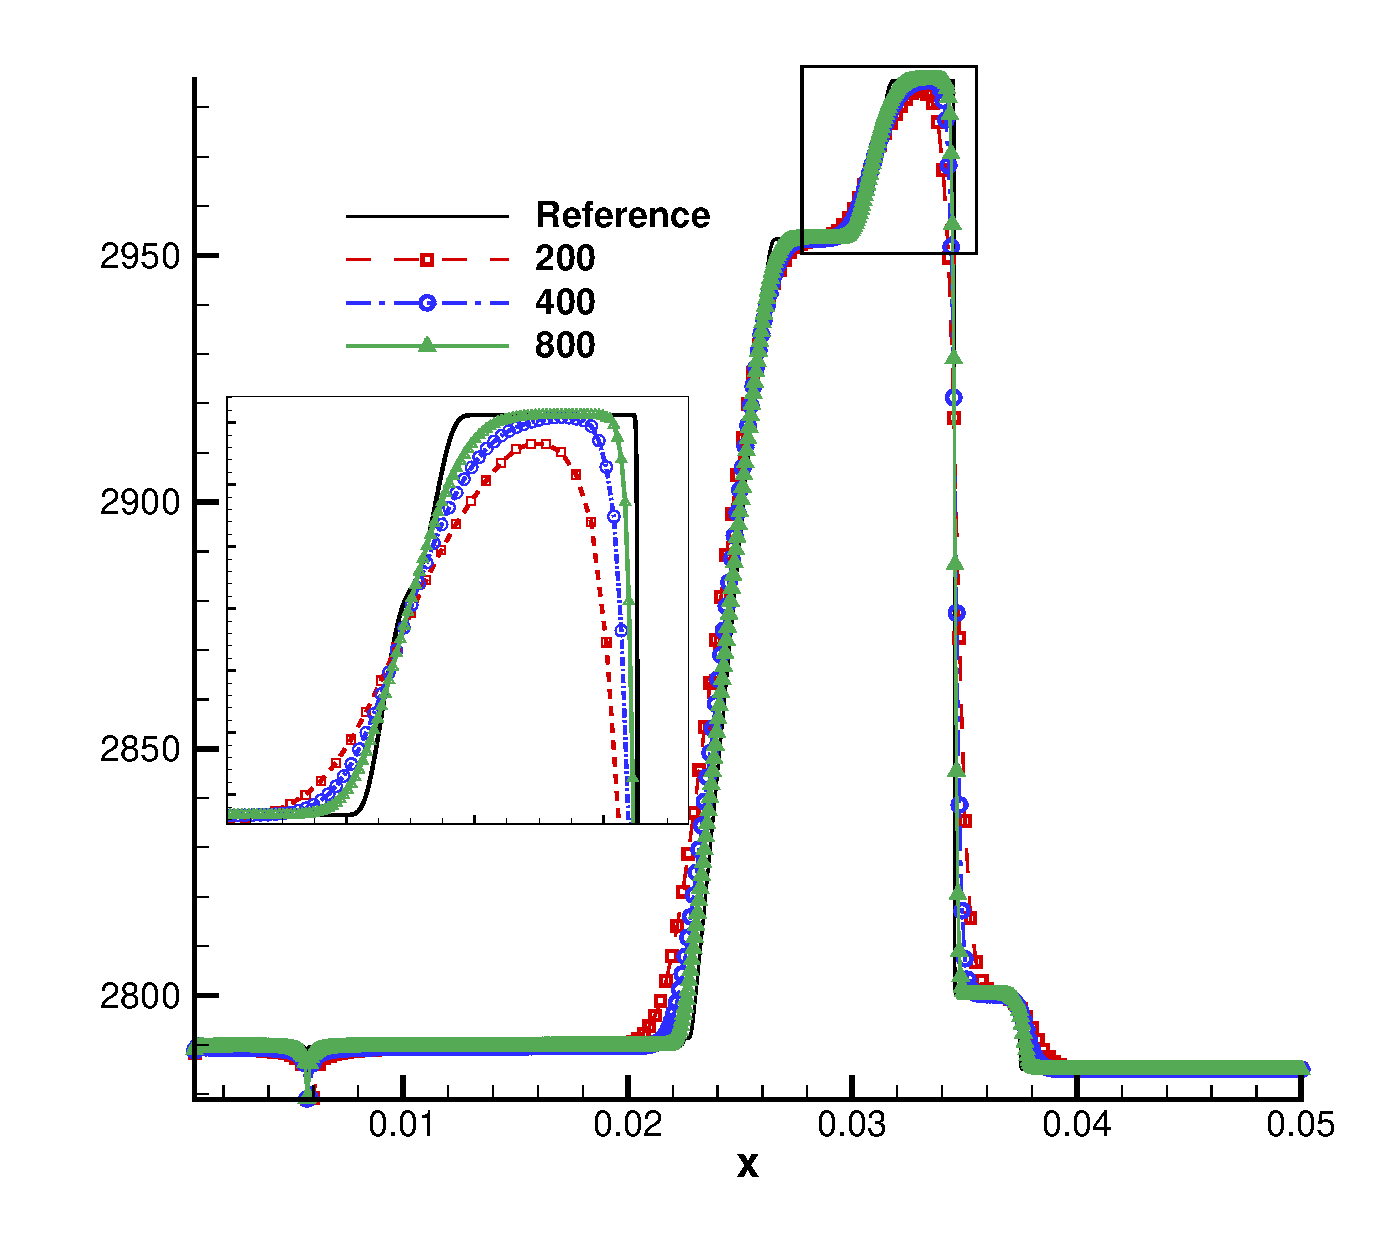
\includegraphics[width = 7cm]{WilkinsRho.eps}};&
	  \node[rectangle](2){
		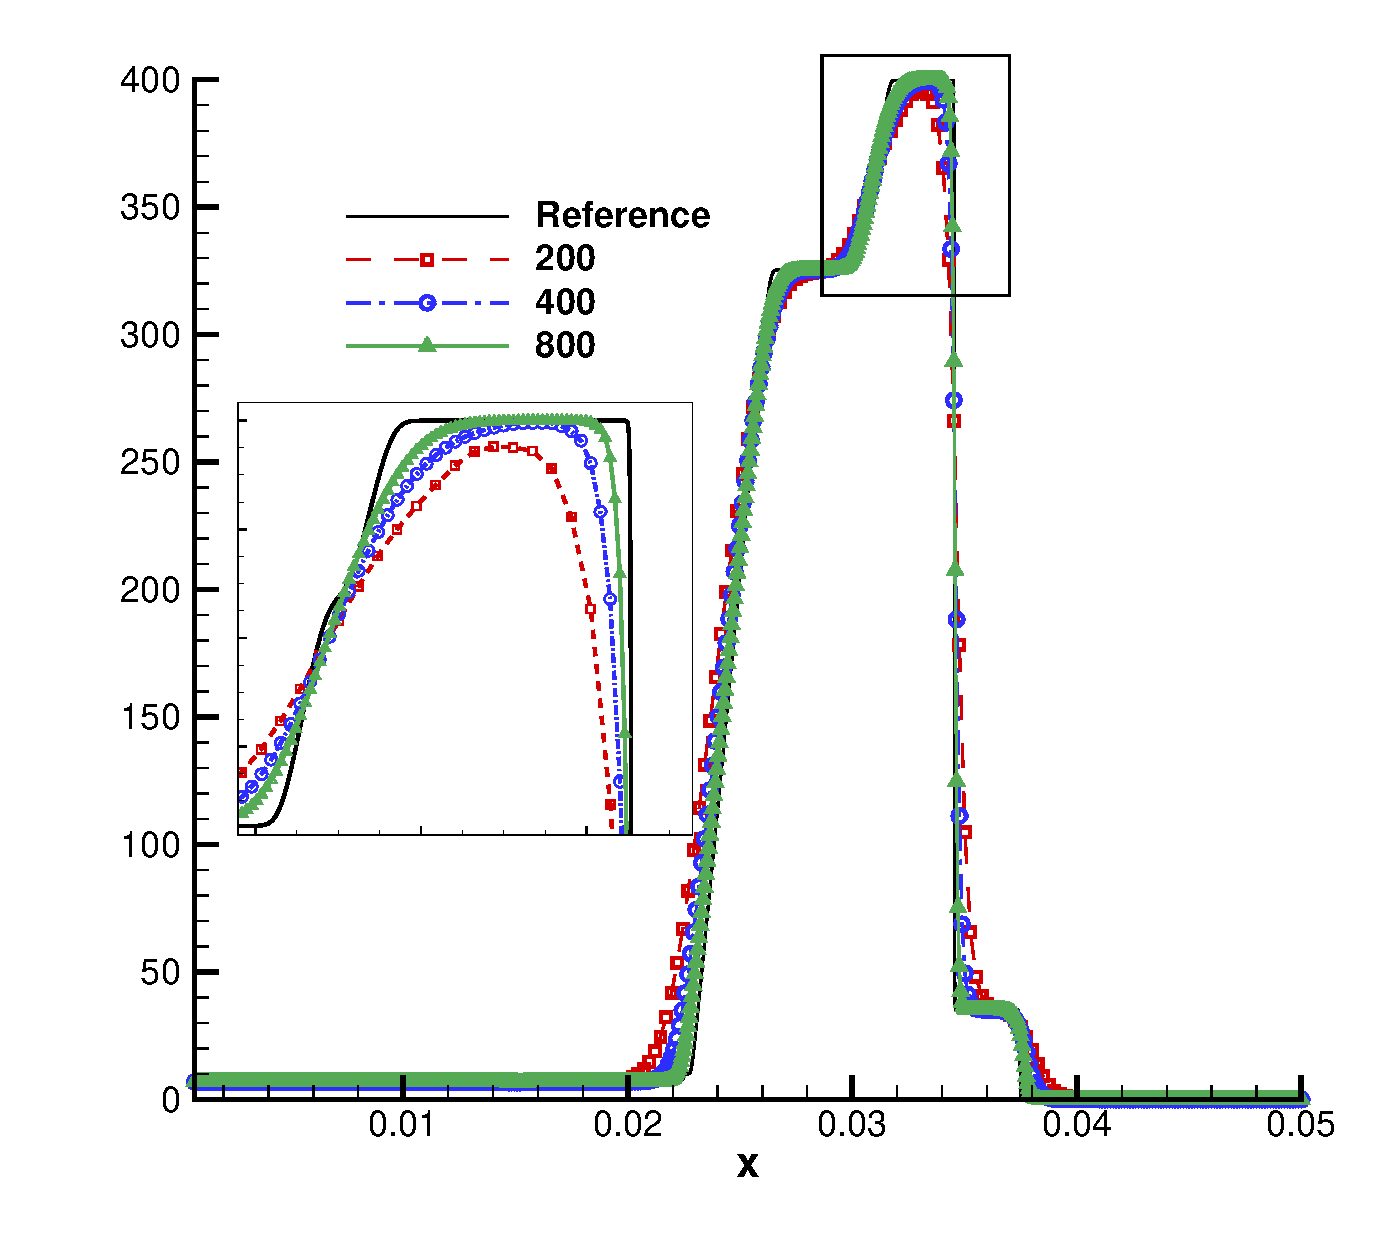
\includegraphics[width = 7cm]{WilkinsU.eps}};\\
	  \node[rectangle](3){
		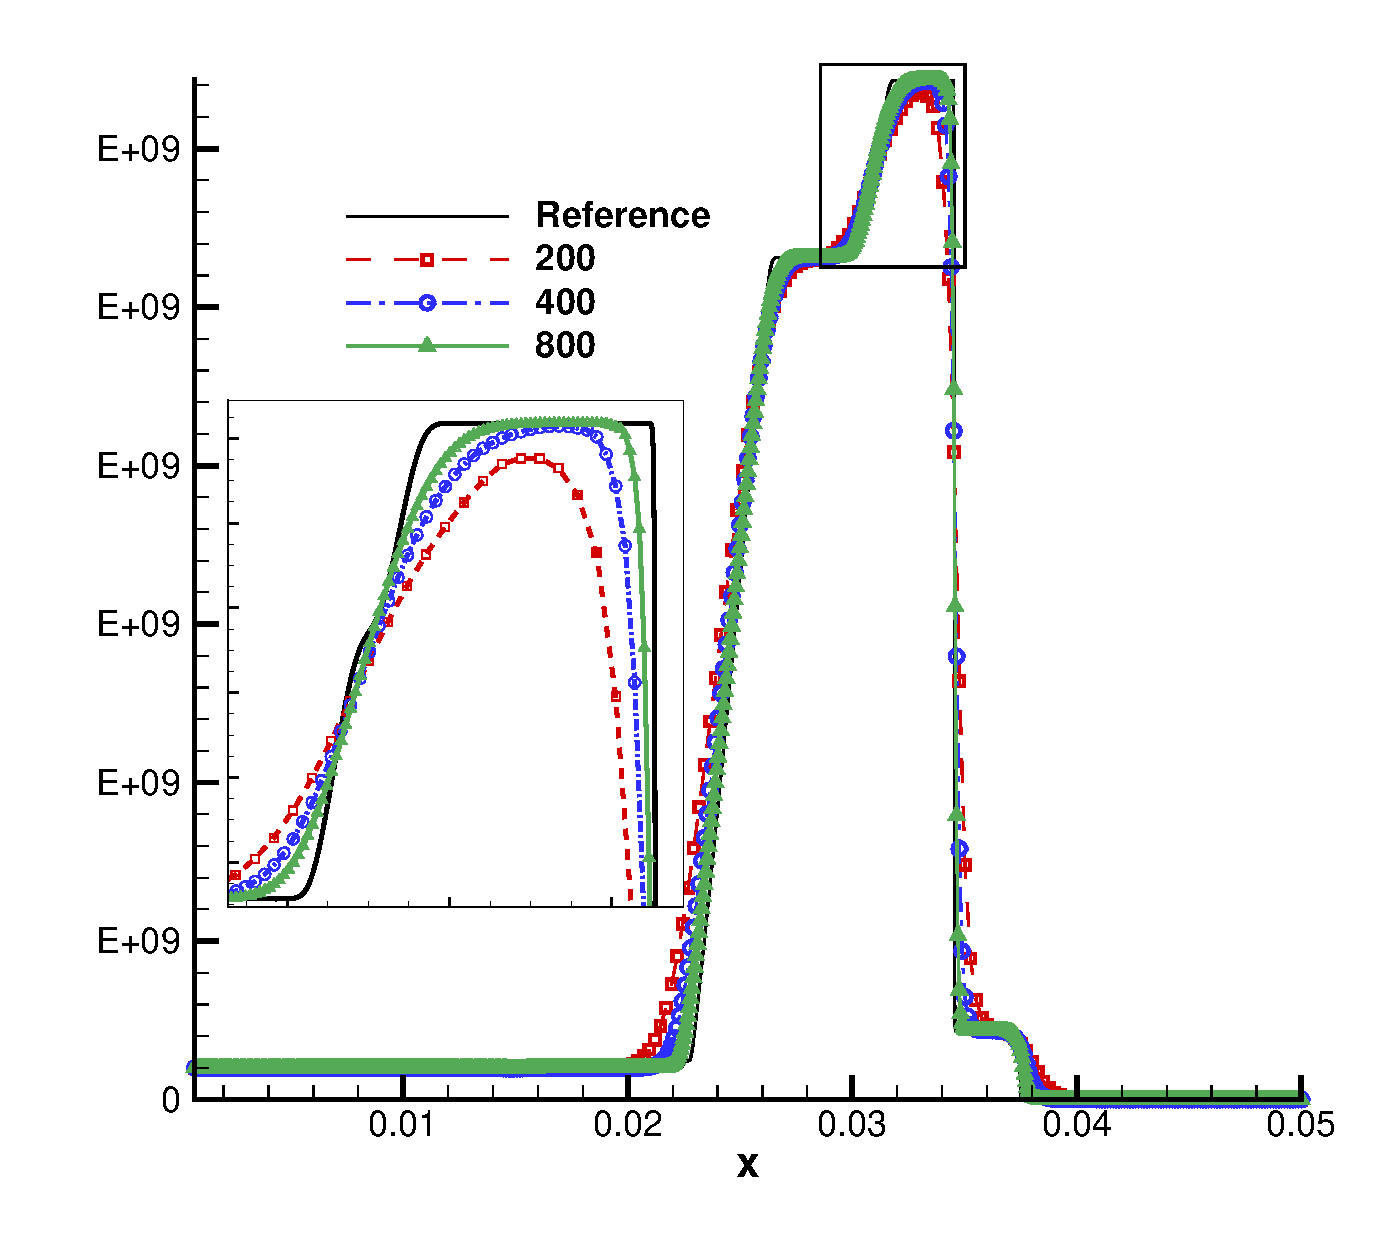
\includegraphics[width = 7cm]{WilkinsP.eps}};&
	  \node[rectangle](4){
		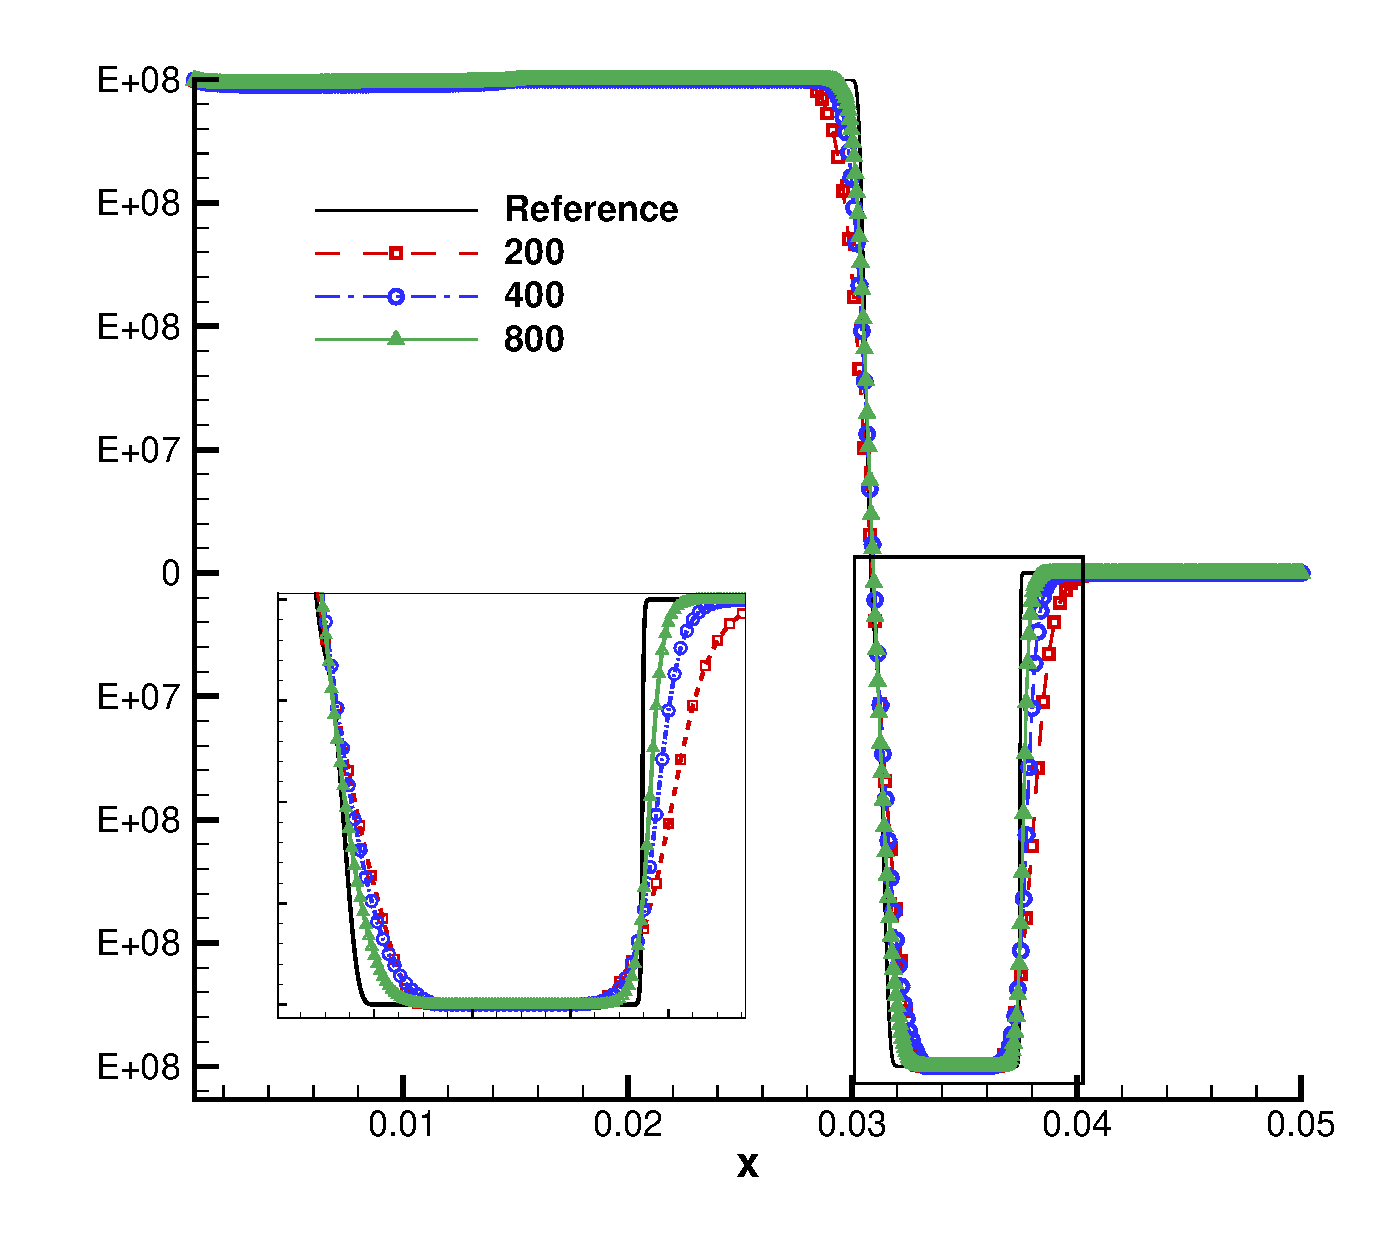
\includegraphics[width = 7cm]{WilkinsSxx.eps}};\\
	  };
	  \node  at (-7,3) [rotate = 90] {$\rho$ ($\text{kg}/\text{m}^3$)};
	  \node at (0.3,3) [rotate = 90]{$u$ ($\text{m}/\text{s}$)};
	  \node  at (-7,-3)[ rotate = 90]{$p$ ($\text{Pa}$)};
	  \node at (0.3,-3)[ rotate = 90]{$s_{xx}$ ($\text{Pa}$)};
	  \end{tikzpicture}
	  \caption{ The result of Wilkins problem}
	  \label{fig:Wilkins1}
	\end{figure}

	\subsection{Multi-material problem 1} \label{pro:multi1}
  Here we consider the multi-material problem without the plasticity effect. A similar case is used in Ref.(\cite{ghaisas2016high}). In this test, a moving  copper stricks on an aluminium plate. The parameters for the EOS and constitutive model for aluminum and copper  are
$ (\rho_0, a_0, \Gamma_0, s, \mu)_{\text{Al}} =(8930 \text{kg}/\text{m}^3, 3940 \text{m}/\text{s},2, 1.49, 2.76 ,2.76\times 10^{10} \text{Pa} )$ and   $(\rho_0, a_0, \Gamma_0, s, \mu)_{\text{copper}} =(2785 \text{kg}/\text{m}^3, 5328 \text{m}/\text{s},2, 1.338,4.5\times 10^{10}\text{Pa})$, respectively. In order to remove the influence of the plasticity effect, we use a very large un-physical yielding strength $Y_0 = 3\times 10^{12} \text{Pa}$.  The initial conditions of this problem are
\begin{equation}\label{eq:initmulti}
  \left\{ \begin{aligned}
	& \rho = 2785 \text{kg}/\text{m}^3, \hspace{0.2cm} u = u_0, \hspace{0.2cm} p = 10^{-12}\text{Pa}, s_{xx} = 0, \hspace{0.2cm} \text{if} \hspace{0.2cm} 0\text{m} \le x \le 2.5\times 10^{-2} \text{m},\\
	&  \rho = 8930 \text{kg}/\text{m}^3, \hspace{0.2cm} u = 0\text{m}/\text{s}, \hspace{0.2cm} p = 10^{-12}\text{Pa}, s_{xx} = 0, \hspace{0.2cm} \text{if} \hspace{0.2cm} 2.5 \times 10^{-2}\text{m} \le x \le 50\times 10^{-2} \text{m}.\\
	\end{aligned}
  \right.
\end{equation}
In this case we take $u_0 = 100 \text{m}/\text{s}$. Figure \ref{fig:multi1}  shows  the numerical results computed by the scheme with HLLCE and the scheme with MHLLCEP at the final time $ t= 2 \times 10^{-6}s$, the reference is given by a refined mesh  with 4000 cells.  We can see there is little difference between the two schemes  for  the multi-material case without plastic waves.
\begin{figure}
  \begin{tikzpicture}
	\matrix[column sep=0mm, row sep = 0mm]
	{
	  \node[rectangle](1){
		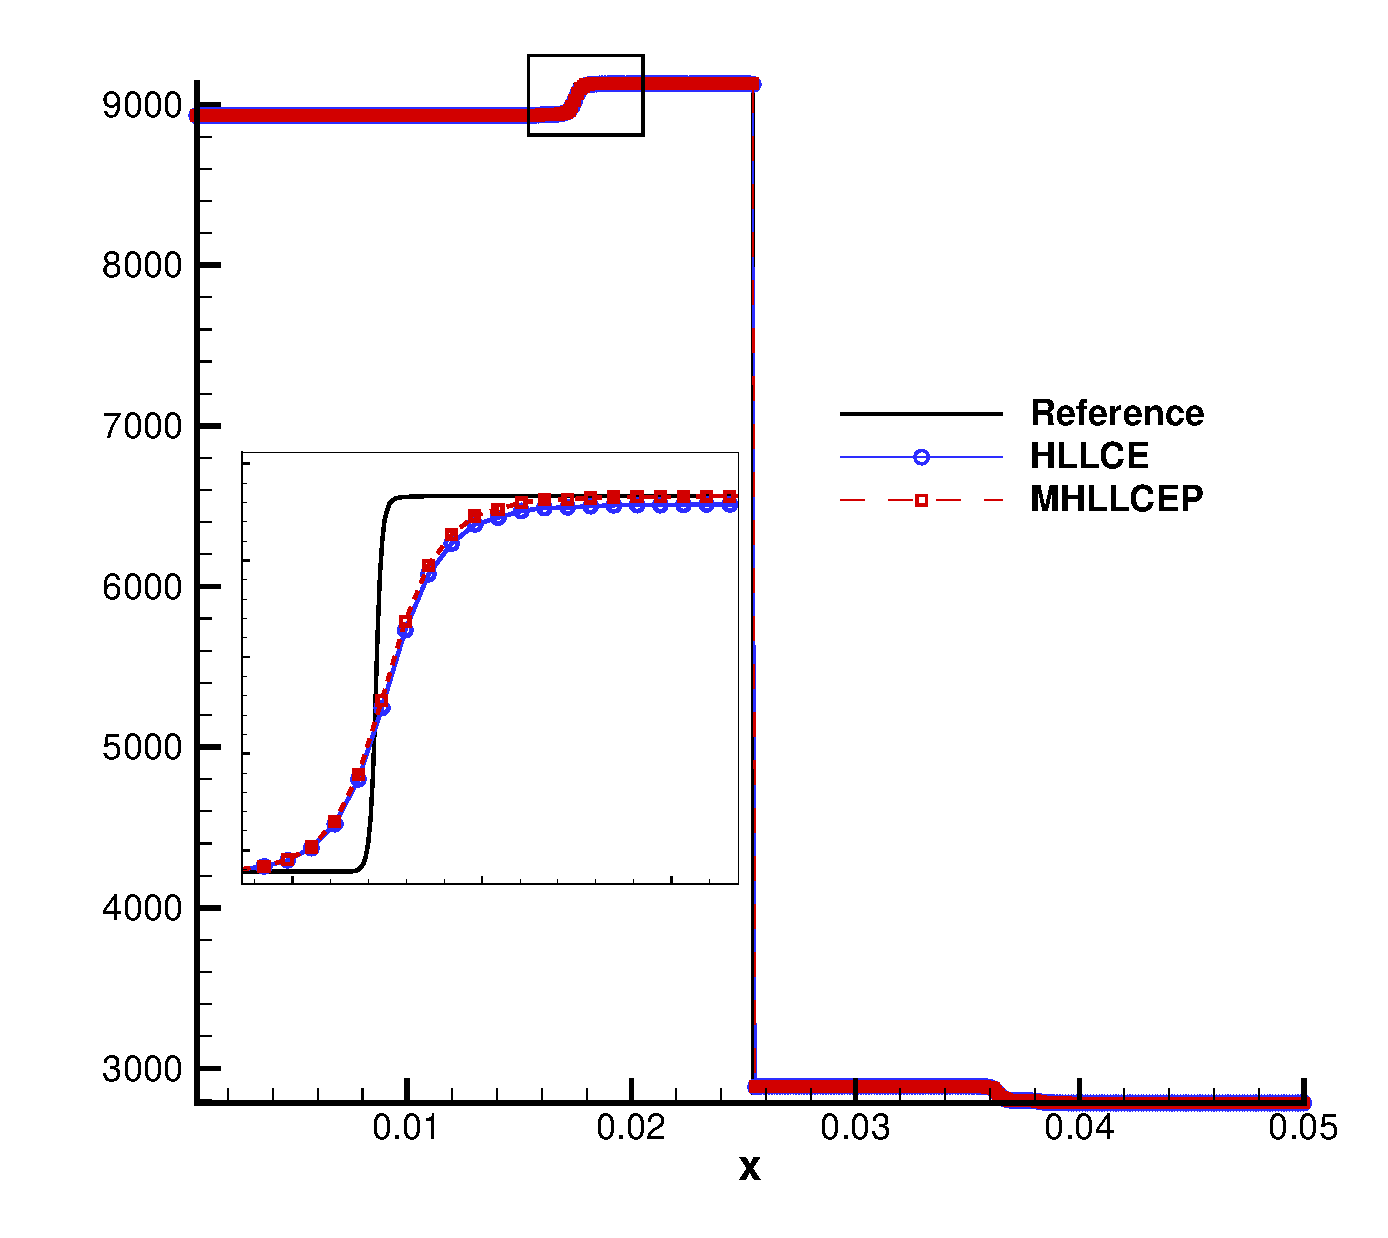
\includegraphics[width = 7cm]{Mult-MaterialsRho.eps}};&
	  \node[rectangle](2){
		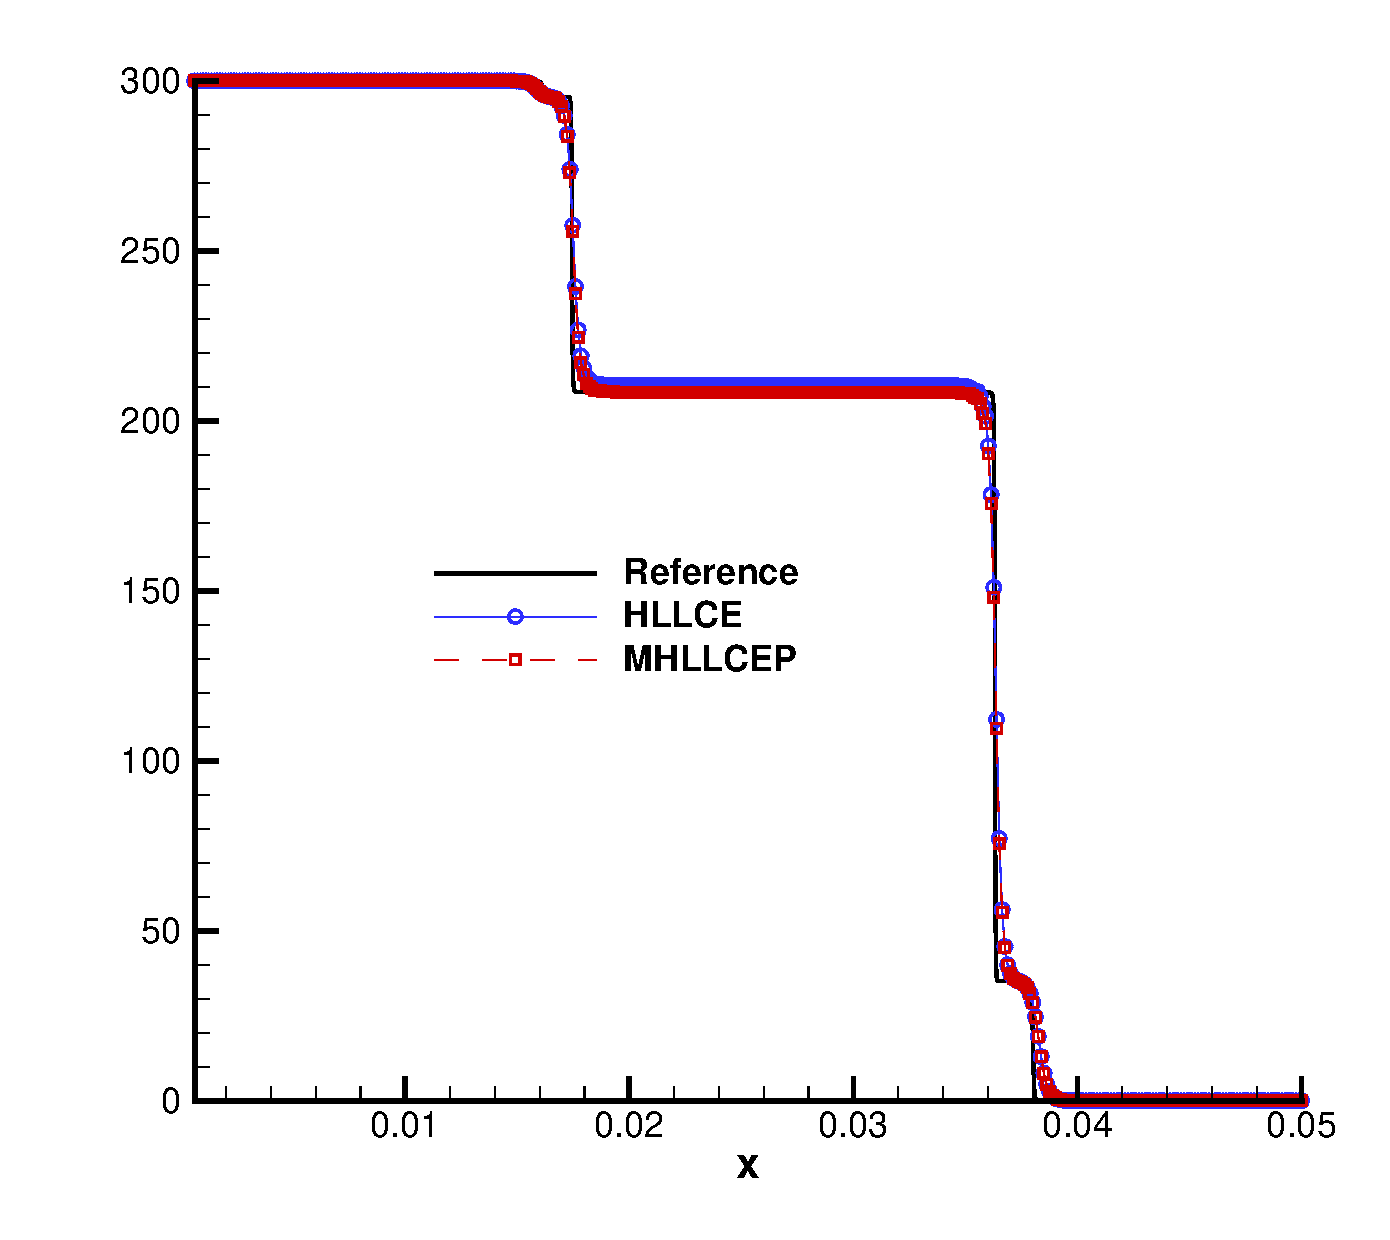
\includegraphics[width = 7cm]{Mult-MaterialsU.eps}};\\
	  \node[rectangle](3){
		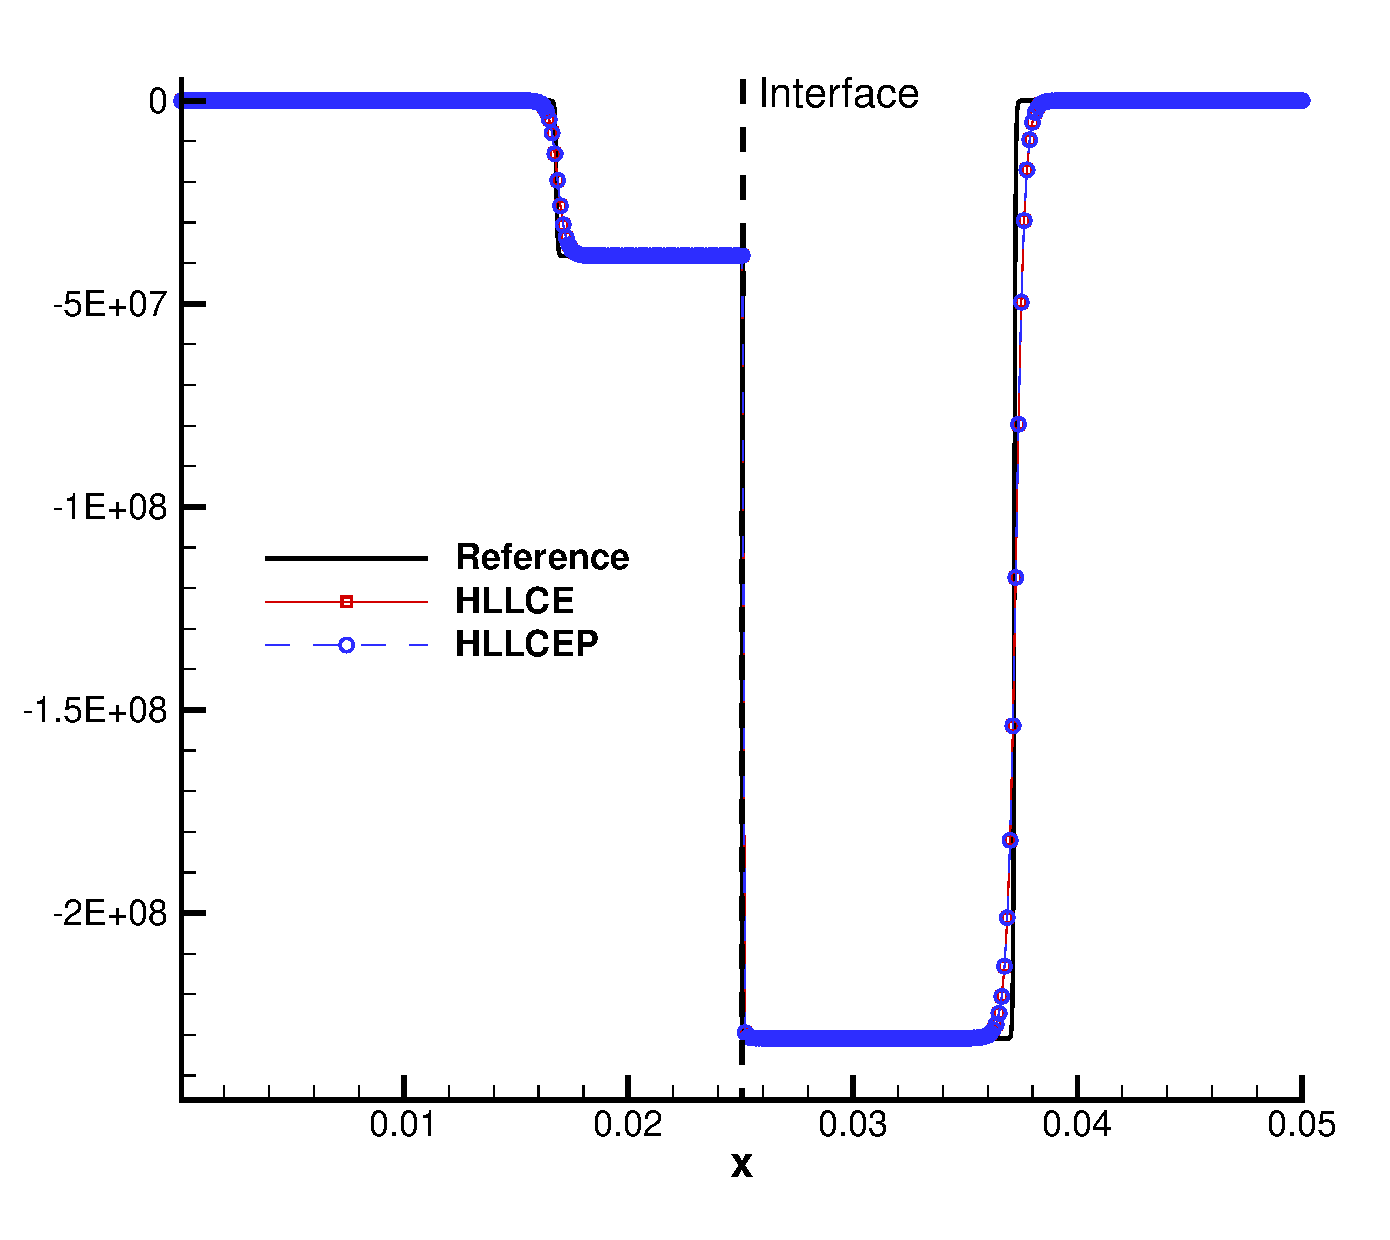
\includegraphics[width = 7cm]{Mult-MaterialsSxx.eps}};&
	  \node[rectangle](4){
		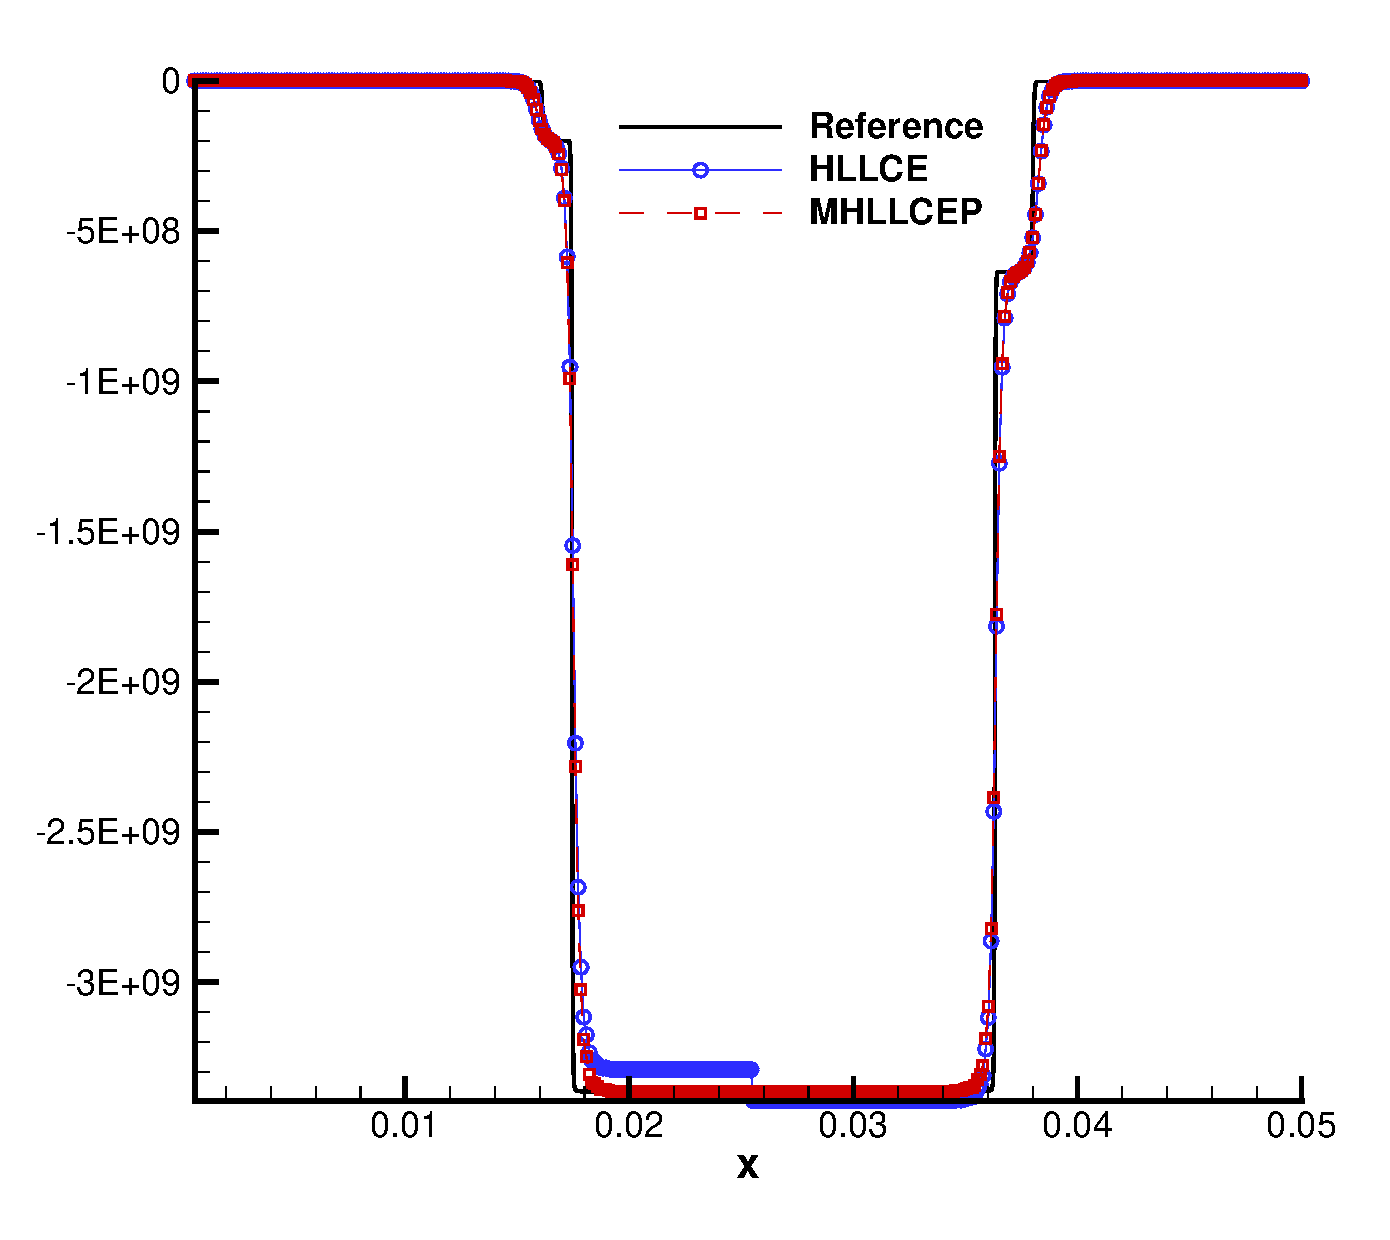
\includegraphics[width = 7cm]{Mult-MaterialsSigma.eps}};\\
	  };
	  \node  at (-7,3) [rotate = 90] {$\rho$ ($\text{kg}/\text{m}^3$)};
	  \node at (0.6,3) [rotate = 90]{$u$ ($\text{m}/\text{s}$)};
	  \node  at (-7,-3)[ rotate = 90]{$p$ ($\text{Pa}$)};
	  \node at (0.6,-3)[ rotate = 90]{$\sigma_{xx}$ ($\text{Pa}$)};
	  \end{tikzpicture}
	  \caption{ The result of two-materials  problem 1}
	  \label{fig:multi1}
	\end{figure}

\subsection{Two materials problem 2}
Next, we consider a similar problem but with plasticity effect. The yield strengths are $Y_0^{\text{Copper}} = 9\times 10^7$ and $Y_0^{\text{Al}} = 3\times 10^8$, respectively. All other  parameters are same to those in problem \ref{pro:multi1}. The initial condition is also same as  Eq.(\ref{eq:initmulti}), we consider this case with a velocity of $u_0 = 60 \text{m}/\text{s}$.
Fig.\ref{fig:multi2} gives the results at final time $ t= 2 \times 10^{-6} \text{s}$ with 200 cell, the solution computed by the scheme with HLLCE is taken as a comparison. The reference solution is given by a refine mesh with 4000 cells. We can see that using HLLCE, the Cauchy stress is not continuous across the interface, which does not confirm with the relation of Eq.(\ref{e28}), while with MHLLCEP, we can get a correct and stable result.
\begin{figure}
  \begin{tikzpicture}
	\matrix[column sep=0mm, row sep = 0mm]
	{
	  \node[rectangle](1){
		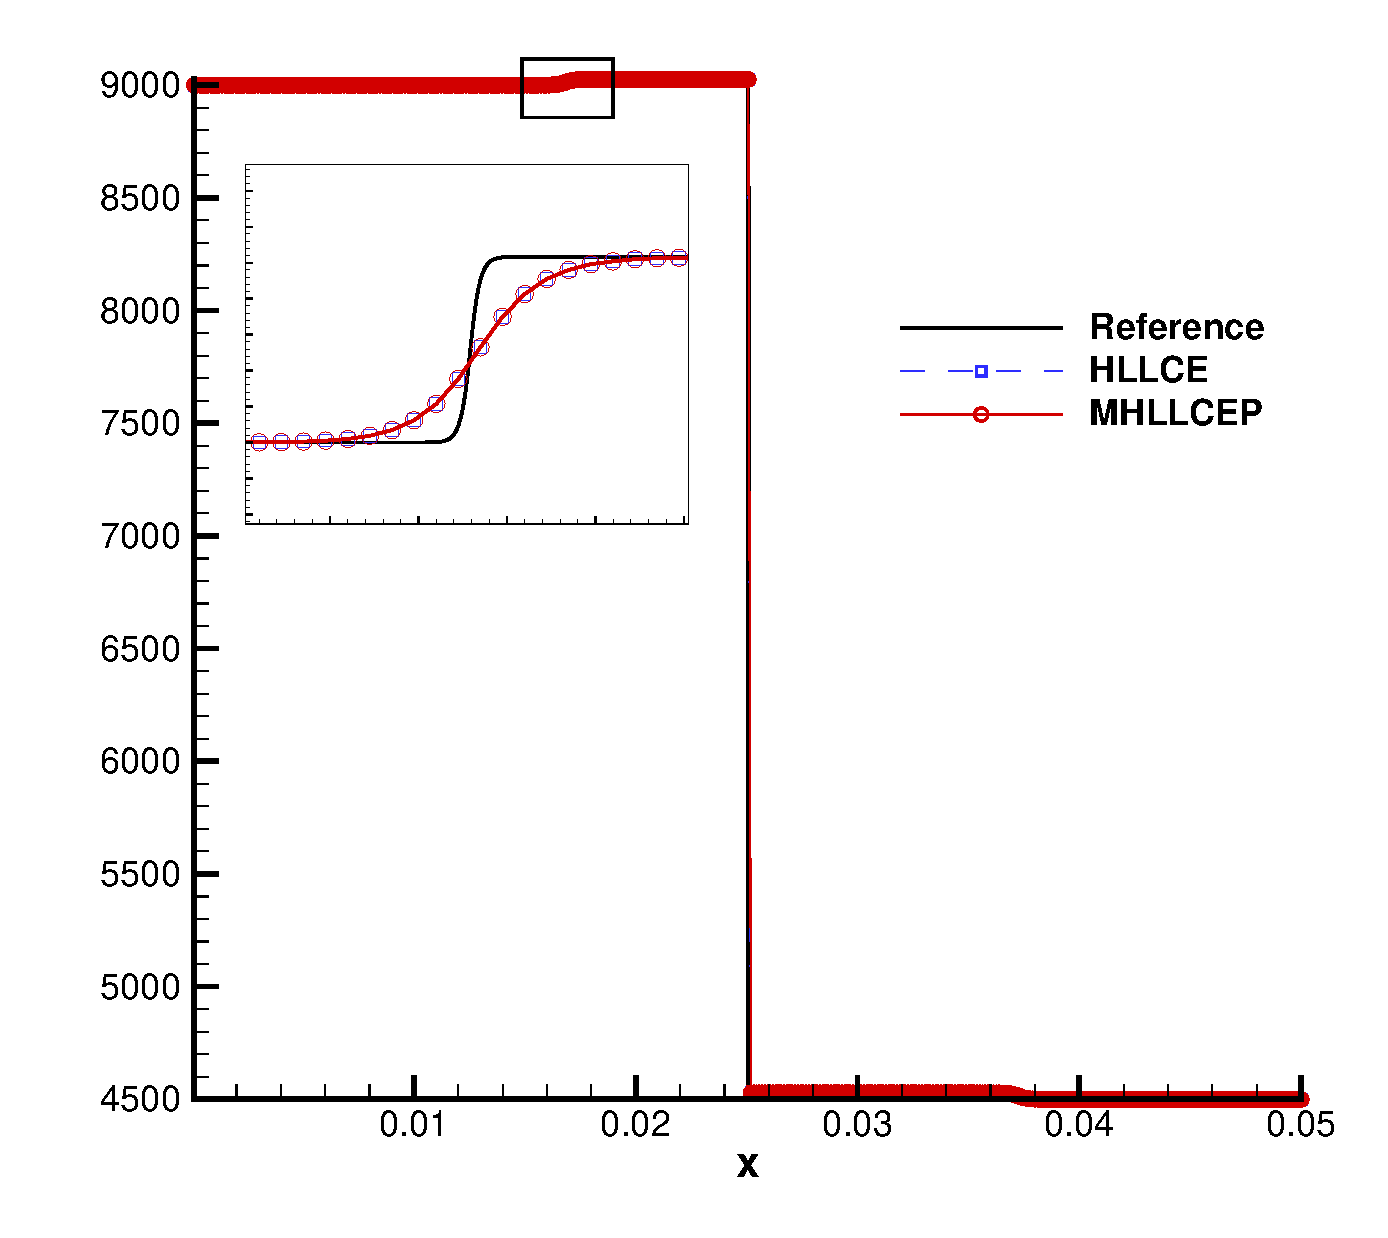
\includegraphics[width = 7cm]{TwoMatterRho.eps}};&
	  \node[rectangle](2){
		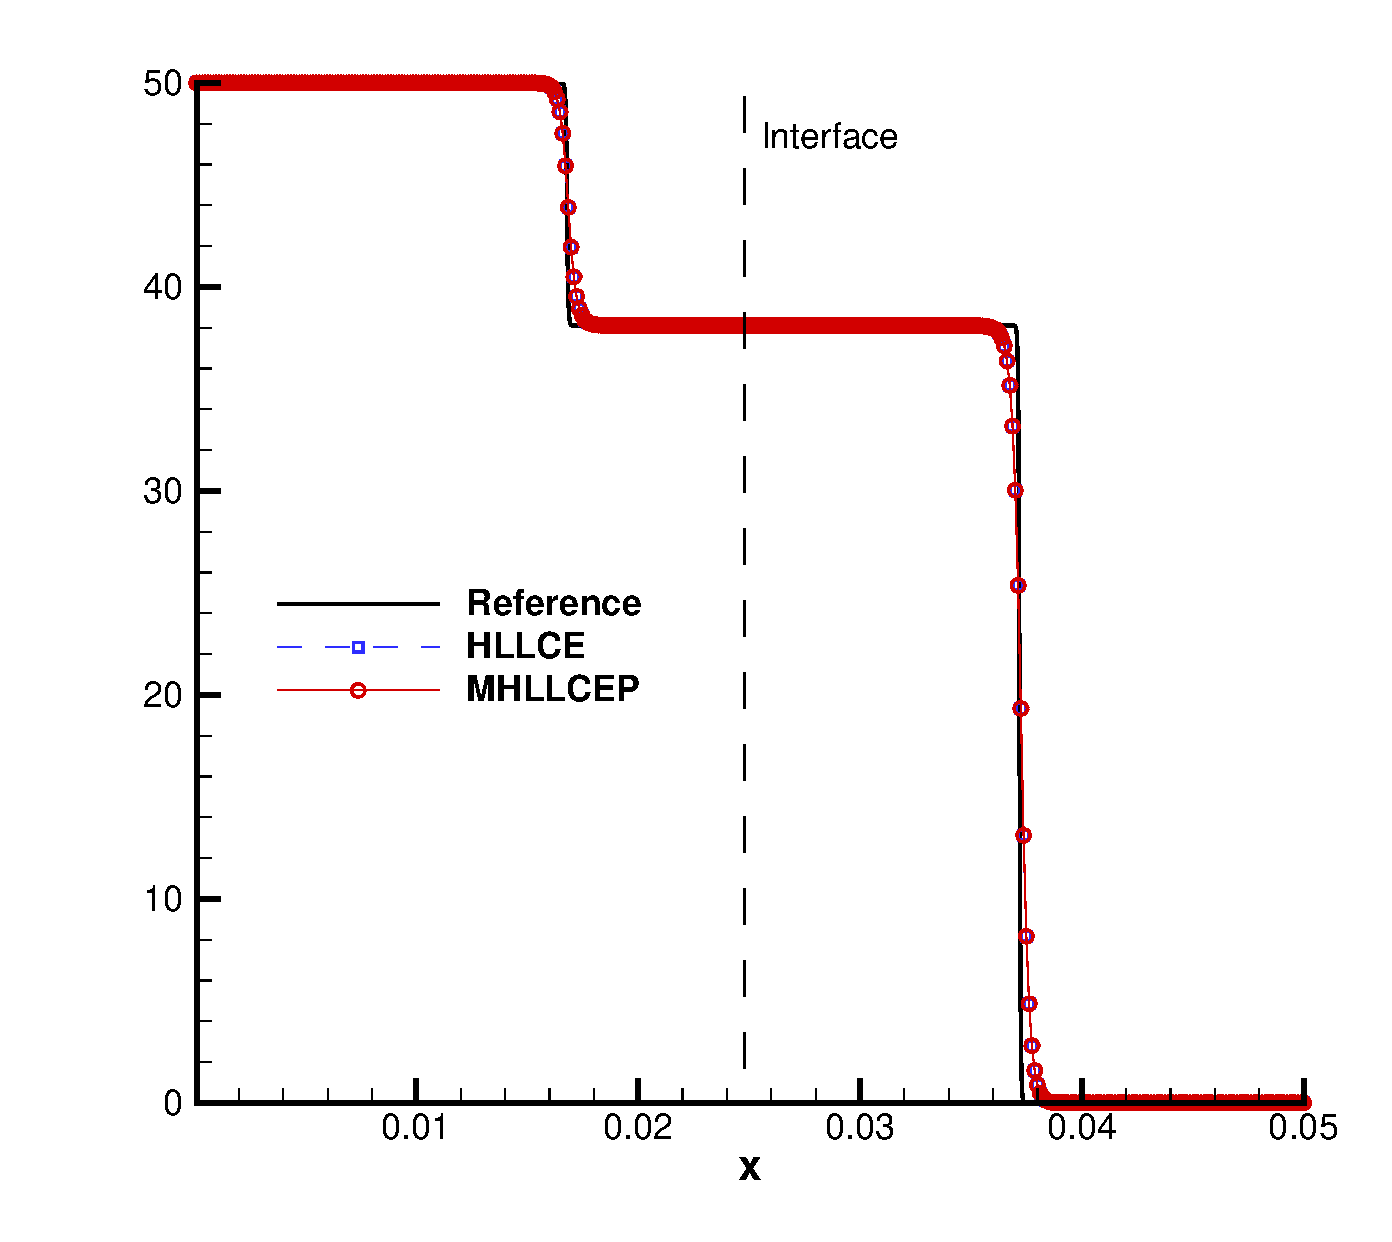
\includegraphics[width = 7cm]{TwoMatterU.eps}};\\
	  \node[rectangle](3){
		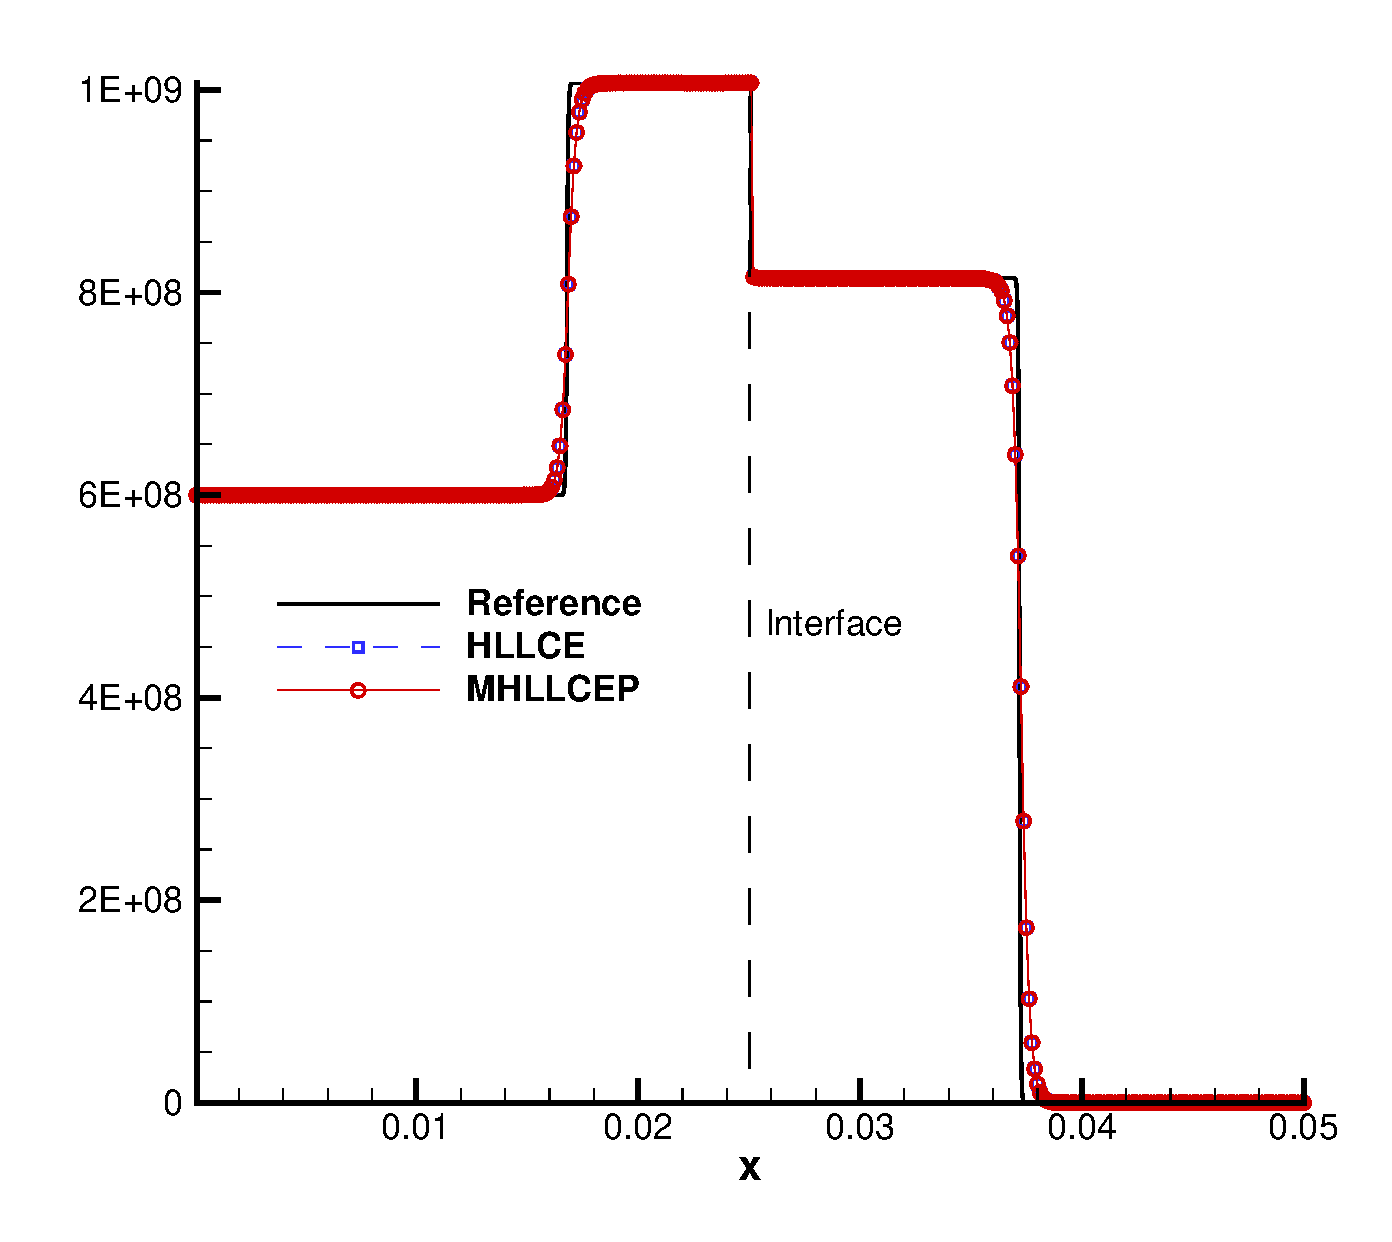
\includegraphics[width = 7cm]{TwoMatterP.eps}};&
	  \node[rectangle](4){
		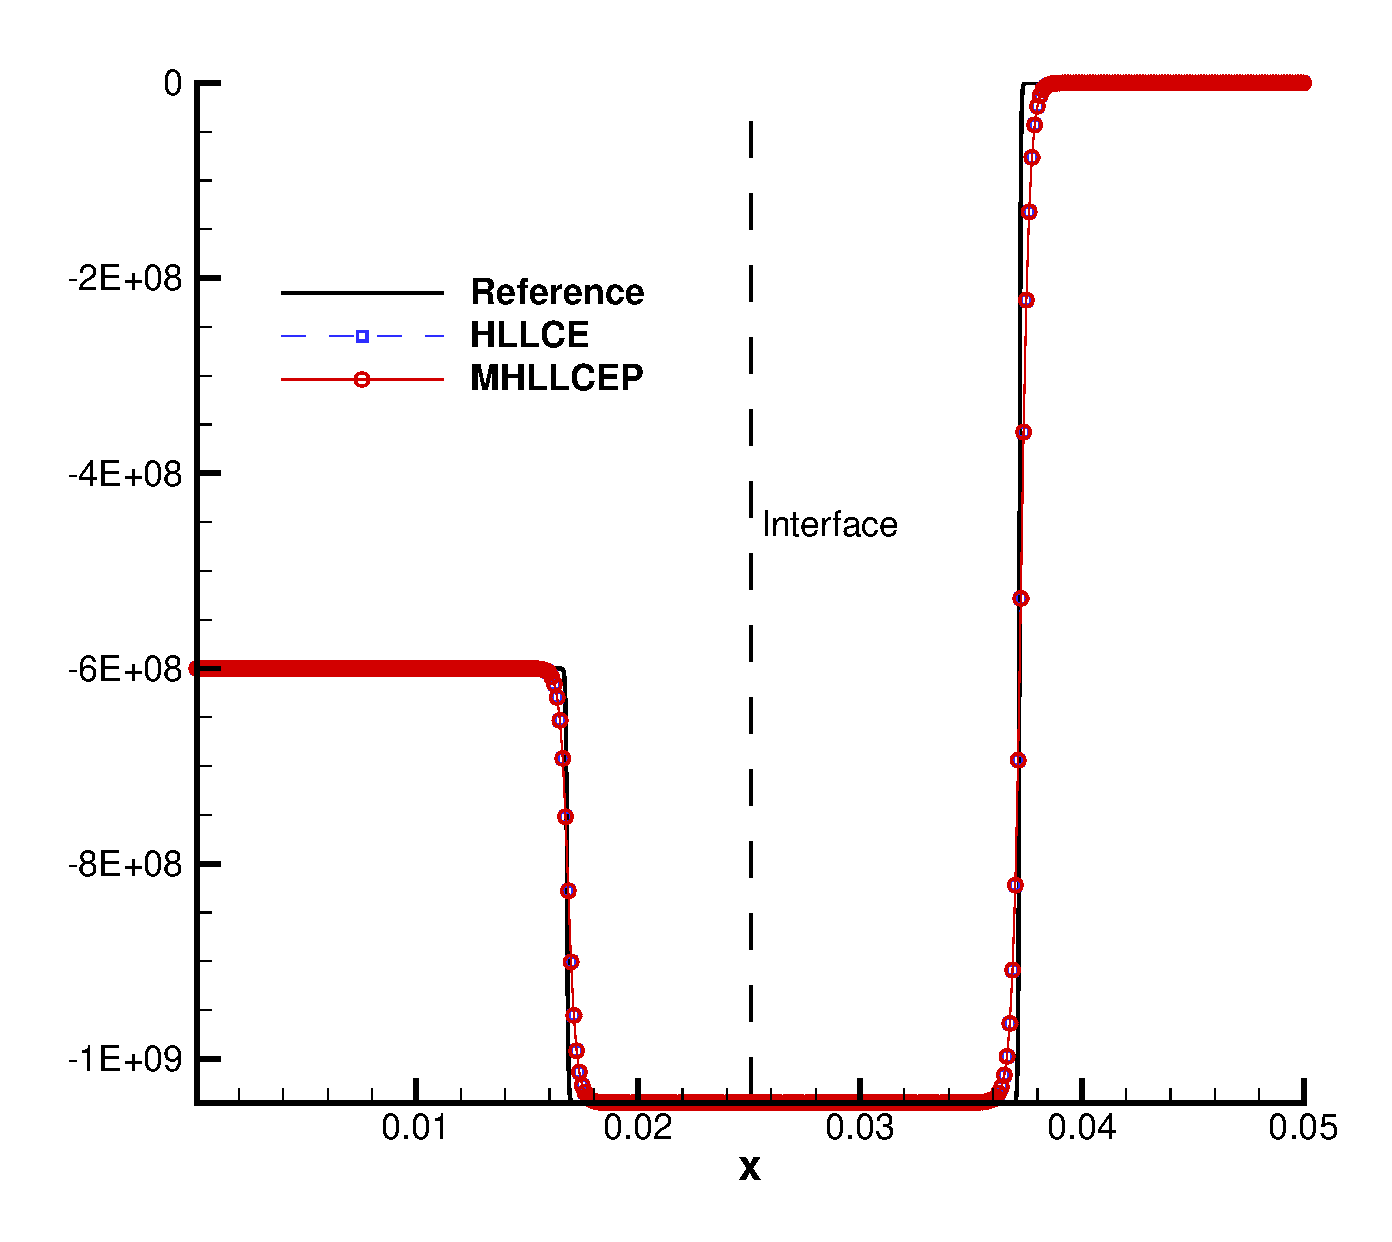
\includegraphics[width = 7cm]{TwoMatterSigma.eps}};\\
	  };
	  \node  at (-7,3) [rotate = 90] {$\rho$ ($\text{kg}/\text{m}^3$)};
	  \node at (0.6,3) [rotate = 90]{$u$ ($\text{m}/\text{s}$)};
	  \node  at (-7,-3)[ rotate = 90]{$p$ ($\text{Pa}$)};
	  \node at (0.6,-3)[ rotate = 90]{$\sigma_{xx}$ ($\text{Pa}$)};
	  \end{tikzpicture}
	  \caption{ The result of two-materials  problem 2}
	  \label{fig:multi2}
	\end{figure}

\section*{Conclutions}
In this paper, a new HLLC-type approximate Reimann solver is constructed to simulate 1D multi-material elastic-plastic flows with the hypo-elastic constitutive model and the von Mises yield criterion. For the elastic-plastic problems with multi-materials, the relations between the interface is difficult to satisfied.  Within  a detail consideration of the plastic waves, there is no unreasonable assumption,  such as  the continuous pressure assumption between the interface, is used in the new HLLCEP method. And thus, the new method can resolve all the  wave structures in multi-material elastic-plasitc problems with accuracy and stability.










%
\section*{Acknowledgement}
This work was supported by NSFC(Grant Nos. 11672047) and Science Challenge Project (Grant No. JCKY2016212A502).



%\section*{References}

\bibliography{mybibfile}

\newpage
  \appendix
  \renewcommand{\appendixname}{Appendix~}
\end{document}
